\documentclass[12pt,a4paper]{report}

\usepackage{styles/dolgozat}

\usepackage{listings}
\usepackage{styles/python}
\usepackage{styles/java}

\usepackage{url}
\usepackage{hyperref}
\hypersetup{breaklinks=true}

\begin{document}

\pagestyle{empty} %a címlapon ne legyen semmi=empty, azaz nincs fejléc és lábléc

% A Miskolci Egyetem címere
{\large
\begin{center}
\vglue 1truecm
\textbf{\huge\textsc{Szakdolgozat}}\\
\vglue 1truecm

\includegraphics[width=4.8truecm, height=4truecm]{images/me_logo.png}\\
\textbf{\textsc{Miskolci Egyetem}}
\end{center}}

\vglue 1.5truecm %függõleges helykihagyás

% A szakdolgozat címe, akár több sorban is
{\LARGE
\begin{center}
\textbf{Automatizált szabadságnyilvántartó rendszer tervezése és megvalósítása WEB-es környezetben.}
\end{center}}

\vspace*{2.5truecm}
% A hallgató neve, évfolyam, szak(ok), a konzulens(ek) neve
{\large
\begin{center}
\begin{tabular}{c}
\textbf{Készítette:}\\
Strutinszky Alex Roland\\
Programtervező informatikus
\end{tabular}
\end{center}
\begin{center}
\begin{tabular}{c}
\textbf{Témavezető:}\\
Dr. Dudás László
\end{tabular}
\end{center}}
\vfill
% Keltezés: Hely, év
{\large
\begin{center}
\textbf{\textsc{Miskolc, 2021}}
\end{center}}

\newpage


\newpage

\pagestyle{empty}

%Feladatkiiras
\begin{flushleft}
\textsc{\bfseries Miskolci Egyetem}\\
Gépészmérnöki és Informatikai Kar\\
Alkalmazott Matematikai Intézeti Tanszék\hspace*{4cm}\hfil \textbf{Szám:}
\end{flushleft}
\vskip 0.5cm
\begin{center}
\large\textsc{\bfseries Szakdolgozat Feladat}
\end{center}
\vskip 0.5cm
Strutinszky Alex Roland (PXMQ3P) programtervező informatikus jelölt részére.\newline

\noindent\textbf{A szakdolgozat tárgyköre:} WEB-es alkalmazás, automatizálás, szabadság, nyilvántartás\newline

\noindent\textbf{A szakdolgozat címe:} Automatizált szabadságnyilvántartó rendszer tervezése és megvalósítása WEB-es környezetben.\newline

\noindent\textbf{A feladat részletezése:}

\medskip

\emph{
	\begin{enumerate}
		\item {Ismerje meg a Miskolci Egyetem Szabályzatának a munkahelyi szabadság kiadására vonatkozó pontjait!}
		\item {Készítse el a rendszertervét egy automatikus havi lejelentések megtételére képes éves szabadságnyilvántartó rendszernek! A program vegye figyelembe a rendes és eseti szabadnapokat, tegye lehetővé a közalkalmazott szabadságválasztásában a maximális szabadságfokot, ugyanakkor tartsa be az összes vonatkozó országos és helyi szabályzat előírását. A rendszer webes felületen, kliens-szerver rendszerben működjön, kezelje az alkalmazotti, vezetői és rendszergazdai jogosultságokat. Nyújtson áttekintő felületet az alkalmazott saját szabadságainak állására, továbbá a vezető számára az összes alkalmazott vonatkozásában.}
		\item {Válassza meg az alkalmas programozási és futtatókörnyezetet a program elkészítéséhez, választását indokolja!}
		\item {Készítse el az alkalmazás programját és minden eshetőségre kiterjedő képzeletbeli adatokkal tesztelje!}
		\item {Készítse el az alkalmazás felhasználói kézikönyvét és ennek kivonatos ismertetésével mutassa be a használat lépéseit!}
	\end{enumerate}
	}

\medskip

\vfill

\noindent\textbf{Témavezető:} Dr. Dudás László PhD (a műszaki tudomány kandidátusa, egyetemi docens) \newline

% \noindent\textbf{Konzulens(ek):} (akkor kötelezõ, ha a témavezetõ nem valamelyik matematikai tanszékrõl való; de persze lehet egyébként is)\newline

\noindent\textbf{A feladat kiadásának ideje: 2018. 09. 01.}\newline

%\noindent\textbf{A feladat beadásának határideje:}

\vskip 2cm

\hbox to \hsize{\hfil{\hbox to 6cm {\dotfill}\hbox to 1cm{}}}

\hbox to \hsize{\hfil\hbox to 3cm {szakfelelős}\hbox to 2cm{}}

\newpage

\vspace*{1cm}  
\begin{center}
\large\textsc{\bfseries Eredetiségi Nyilatkozat}
\end{center}
\vspace*{2cm}  

Alulírott \textbf{Strutinszky Alex Roland}; Neptun-kód: \texttt{PXMQ3P} a Miskolci Egyetem Gépészmérnöki és Informatikai Karának végzős Programtervező informatikus szakos hallgatója ezennel büntetőjogi és fegyelmi felelősségem tudatában nyilatkozom és aláírásommal igazolom, hogy \textit{Automatizált szabadságnyilvántartó rendszer tervezése és megvalósítása WEB-es környezetben.}
című szakdolgozatom saját, önálló munkám; az abban hivatkozott szakirodalom
felhasználása a forráskezelés szabályai szerint történt.\\

Tudomásul veszem, hogy szakdolgozat esetén plágiumnak számít:
\begin{itemize}
\item szószerinti idézet közlése idézőjel és hivatkozás megjelölése nélkül;
\item tartalmi idézet hivatkozás megjelölése nélkül;
\item más publikált gondolatainak saját gondolatként való feltüntetése.
\end{itemize}

Alulírott kijelentem, hogy a plágium fogalmát megismertem, és tudomásul veszem, hogy
plágium esetén szakdolgozatom visszautasításra kerül.

\vspace*{3cm}

\noindent Miskolc, \hbox to 2cm{\dotfill} .év \hbox to 2cm{\dotfill} .hó \hbox to 2cm{\dotfill} .nap

\vspace*{3cm}

\hspace*{8cm}\begin{tabular}{c}
\hbox to 6cm{\dotfill}\\
Hallgató
\end{tabular}



\newpage

\noindent 1.

\begin{tabular}{cl}
&szükséges (módosítás külön lapon) \\
A szakdolgozat feladat módosítása& \\
& nem szükséges\\
&\\
\hbox to 4cm{\dotfill}&\multicolumn{1}{c}{\hbox to 5cm{\dotfill}}\\
dátum& \multicolumn{1}{c}{témavezető(k)}
\end{tabular}
\vskip1.5mm

\noindent 2. A feladat kidolgozását ellenőriztem:

\vskip1.5mm

\begin{tabular}{l@{\hspace*{4cm}}l}
témavezető (dátum, aláírás):& konzulens (dátum, aláírás):\\
\dotfill&\dotfill\\
\dotfill&\dotfill\\
\dotfill&\dotfill
\end{tabular}

\vskip1.5mm

\noindent 3. A szakdolgozat beadható:

\vskip1.5mm

\begin{tabular}{@{\hspace*{1.3cm}}c@{\hspace*{2.1cm}}c}
\hbox to 4cm{\dotfill}&\multicolumn{1}{c}{\hbox to 5cm{\dotfill}}\\
dátum& \multicolumn{1}{c}{témavezető(k)}
\end{tabular}

\vskip1.5mm

\noindent 4.
\begin{tabular}[t]{@{}l@{\hspace*{1mm}}l@{\hspace*{1mm}}l@{}}
A szakdolgozat& \hbox to 3.5cm{\dotfill} &szövegoldalt\\
              & \hbox to 3.5cm{\dotfill} &program protokollt (listát, felhasználói leírást)\\
              &\hbox to 3.5cm{\dotfill}   &elektronikus adathordozót (részletezve)\\
              &\hbox to 3.5cm{\dotfill} & \\
              &\hbox to 3.5cm{\dotfill} &egyéb mellékletet (részletezve)\\
              &\hbox to 3.5cm{\dotfill} &\\
\end{tabular}
\newline tartalmaz.

\vskip1.5mm

\begin{tabular}{@{\hspace*{1.3cm}}c@{\hspace*{2.1cm}}c}
\hbox to 4cm{\dotfill}&\multicolumn{1}{c}{\hbox to 5cm{\dotfill}}\\
dátum& \multicolumn{1}{c}{témavezető(k)}
\end{tabular}

\noindent 5.

\begin{tabular}{ll}
&bocsátható\\
A szakdolgozat bírálatra& \\
& nem bocsátható\\
\end{tabular}

\vskip1.5mm

\noindent A bíráló neve: \hbox to 8cm{\dotfill}

\vskip4mm

\begin{tabular}{@{\hspace*{1.3cm}}c@{\hspace*{2.1cm}}c}
\hbox to 4cm{\dotfill}&\multicolumn{1}{c}{\hbox to 5cm{\dotfill}}\\
dátum& \multicolumn{1}{c}{szakfelelős}
\end{tabular}

\noindent 6.
\begin{tabular}[t]{@{}l@{\hspace*{1mm}}l@{\hspace*{1mm}}l@{}}
A szakdolgozat osztályzata& &\\
&a témavezető javaslata:& \hbox to 3cm{\dotfill}\\
&a bíráló javaslata:& \hbox to 3cm{\dotfill}\\
&a szakdolgozat végleges eredménye:& \hbox to 3cm{\dotfill}
\end{tabular}

\vspace*{4mm}

\noindent Miskolc, \hbox to 4.5cm{\dotfill} \hspace*{2.5cm}
\begin{tabular}[t]{cc}
\hbox to 6cm{\dotfill}\\
a Záróvizsga Bizottság Elnöke
\end{tabular}


\cleardoublepage
\pagenumbering{gobble}
\tableofcontents
\cleardoublepage
\pagenumbering{arabic}

\newpage

\pagestyle{fancy}

\Chapter{Bevezetés}

A 21. században az eddigieknél, sokkal nagyobb fejlődést mutató, egyre inkább digitalizálódó világban a különböző akár mindennapi adminisztrációk egyre nagyobb részét végezzük digitális felületeken.
A papír alapú formanyomtatványokat már több helyen leváltották, a dinamikusan fejlődő és könnyedén változtatható WEB-es felületek. A dossziékat és irattartókat pedig adatbázisokra cserélték.
Ezáltal új lehetőségek nyíltak a munkáltatók számára, hogy a bonyolult, időigényes, személyes ügyintézést igénylő műveleteket különböző szoftvereken keresztül végezzék el.

Mivel egy nagyobb szervezetben a munkavállalók száma akár a több százat is elérheti, és ezekre a személyekre meglehet, hogy külön szabályok vonatkoznak így szükségessé vált a szabadság nyilvántartó rendszerek bevezetése.
Ezt az igényt természetesen hamar sikerült kielégíteni, de a piacon található szolgáltatások általános megoldást kínálnak amik a lehető legtöbb szervezeti egységre alkalmazhatóak és a legelterjedtebb szabályozásokat fedik le csupán.

Ezeket az igényeket eleinte jól megtervezett excel táblák és sablonok elégítették ki, de idővel ezek bonyolulttá és nehezen követhetővé váltak, valamint kimondottan sok helyet foglaltak. nem kellett sok idő, hogy a WEB applikációk megjelenésével és széles körben elterjedésével, több piac orientált rendszer szülessen.

A létező megoldások általánossága miatt, nem lehet specifikusan egy adott ország törvényeire alkalmazva konfigurálni, így a megannyi eltérő szabályozás miatt minden évben az alkalmazott számára elérhető szabadnapok kiszámolása, és jóváírása többnyire kézzel történik. Továbbá felmerül az a probléma is, hogy amennyiben egy alkalmazottra, vagy szervezeti egységre nem ugyanazok a szabályok vonatkoznak, abban az esetben milyen beállítások érhetőek el a különbségek kezelésére? Ezt a kérdést megválaszolva azt vesszük észre, hogy jelenleg nem elérhető olyan WEB-es szoftver ami alkalmazható vagy akár, automatizálható egy Magyar felsőoktatási intézményben, anélkül, hogy az eddigi papírmunkát maradéktalanul leváltsa. Ezáltal a felhasználók kénytelenek nehezen átlátható módon igényelni és a követni az elérhető és felhasznált szabadságaikat.

Az egyetemeken központosított nyilvántartást vezetnek az alkalmazottak szabadságairól, de ezzel kapcsolatban a következő kérdések merülnek fel: Vajon minden alkalmazottra egyforma jogszabályok érvényesek? A különböző jogszabályokat, képes külön kezelni a rendszer? Mennyire hozzáférhető ez az alkalmazottak számára? Nyomon tudják követni egyszerűen a felhasznált és hátralévő szabadnapjaikat az emberek? Mennyi időt vesz el tőlük egy ilyen ügyintézés? Van olyan lehetőség ami mindenkinek megfelel?

Ezen kérdéskört kutatva a dolgozatom célja, hogy tervezzek és megvalósítsak egy olyan WEB-es felületen elérhető alkalmazást, ami egy központi szerverre telepítve, majd a megfelelő beállítások után, lehetővé teszi, hogy a Magyar szabályozásoknak megfelelően a felhasználók képesek legyenek gond nélkül naprakész információhoz jutni a szabadságaikkal kapcsolatban. Valamint a rendelkezésre álló adatok alapján a lehető legnagyobb mértékben automatizáljam a rendszert. 

Dolgozatom során részletesen utánajártam az országunkban létező szabadság típusoknak, ezekhez kapcsolódó feltételeknek, valamint az átlagostól eltérő munkakörökre vonatkozó szabályozásoknak és implementáltam egy általam tervezett megoldást. Az implementáció során a próbáltam céges körülményeket szimulálni és a lehető legmodernebb technikai megoldásokkal dolgozni. Szakdolgozatom a bonyolult struktúra, az eltérő vagy akár változó statisztikai lehetőségek és az igényes megvalósítás időigényessége miatt nem tér ki a felsőoktatásban dolgozó közalkalmazottakra nem releváns pótszabadságokra valamint a szülési szabadság kimondottan bonyolult lehetséges kimeneteleire, csak és kizárólag az ideális esetre, továbbá a megvalósítás esetén: statisztikai funkciókra, a felettesi jóváhagyásra, valamint a felületre. Az felsorolt működési elemekre csak elméleti, rendszertervezés szintjén tér ki.

A kutatás és az implementáció remélhetőleg választ ad arra, hogy lehetséges-e megvalósítani teljesen automatizált szabadságnyilvántartó applikációkat, valamint az általam megírt szoftver milyen további fejlesztésekkel, alkalmazható akár napi szinten a Magyar egyetemek tanszékein dolgozó oktatók, adminisztrátorok és egyéb munkakörökben dolgozók átláthatóbb szabadság menedzsmentjének érdekében.  
\Chapter{Magyar felsőoktatási szabadságnyilvántartó szoftverszolgáltatás fejlesztése}

Célszoftver fejlesztése esetén a szoftver fejlesztést megelőzi egy kutatás és igény felmérés, ami során feltérképezzük a felhasználói igényeket, és az ezekhez tartozó elérhető kínálatot. Az igényeknek megfelelően pedig új hasznos funkciókat adunk a saját programunkhoz.

A felhasználók tökéletes forrást biztosítanak az ötletek és igények kialakításához, viszont ezeknek a megértéséhez, megvalósításához szükség van háttér ismeretekre is mint például jogszabályok és alap fogalmak. Amik alapján megtervezhető a program struktúrája, és működése is jobban leírható.

Miután megvan a szükséges tudás, a célnak megfelelően technológiai eszköztárat kell választanunk, valamint tudnunk kell milyen fejlesztési metodológiát alkalmazunk a feladatok és eredmények nyomon követésére. 

Ez a fejezet felvázolja, az elérhető lehetőségek hiányosságait a Magyar felsőoktatásban dolgozók mint felhasználók szempontjából, definiálja a témakörben használatos elméleti fogalmakat, valamint részletesen bemutatja a választott technológiai eszköztárat és folyamatokat.

\Section{Fogalmak, törvények, meghatározott feltételek}

Fontos, hogy tisztában legyünk a tervezés során számunkra lényeges meghatározásokkal, szabályokkal. A fejezet ezen részében a tervezés szempontjából szükséges, a munkatörvénykönyvében definiált fogalmakat, szabályozásokat mutatom be.

\subsection{Szabadság}

A szabadság olyan napok összessége, melyet a munkavállaló szerződésében foglalt munkanap helyett, munkahelyétől és a munkavégzéstől távol tölt. A tervezett szabadnapokat, a munkáltató felé, a munkavállalónak meghatározott idővel előre kell jelezni. Mind a két félre vonatkozó törvények, ész szabályozások akár évente változhatnak így követnünk kell az aktuális évben érvényes kiadásokat.

A szabadságnak két fajtája van:
\begin{itemize}
	\item \textbf{Fizetett\footnote{A dolgozat későbbi részében részletes bemutatásra kerül.}:} Szintén két részre bontható, munkanapnak minősül, szabályok alapján előre definiált, a munkavállaló pihenését és regenerálódását szolgálja. 
	\item \textbf{Fizetés nélküli:} A fizetett szabadságon felül igénybe vett szabadnapok, alapos indokkal vagy közös megegyezés esetén élhet vele a munkavállaló, ezekre a napokra nem köteles a munkáltató fizetést biztosítani. \cite{fizetesNelkuliSzabadsag}
\end{itemize}

\subsection{Fizetett szabadság}

A fizetett szabadság definíciója: 

"A szabadságnak a munkavállaló pihenését, regenerálódását szolgáló rendeltetéséből következik, hogy az alapvetően a ténylegesen munkában töltött idő után illeti meg a munkavállalót minden naptári évben. Mindazonáltal a törvény tényleges munkavégzés hiányában is munkában töltött – így szabadságra jogosító – időnek minősíti a következő időtartamokat:
\begin{itemize}
\item a munkaidő-beosztás alapján történő munkavégzési kötelezettség alóli mentesülés időtartama (ilyennek minősülnek például a pihenőnapok, pihenőidők vagy a rendkívüli munkavégzés ellenértékeként biztosított szabadidő),
\item a szabadság időtartama,
\item a szülési szabadság időtartama,
\item a gyermek gondozása céljából igénybe vett fizetés nélküli szabadság első hat hónapja,
\item a naptári évenként harminc napot meg nem haladó keresőképtelenség (a naptári évre eső egyes keresőképtelenségek tartamát össze kell számítani),
\item a tényleges önkéntes tartalékos katonai szolgálatteljesítés három hónapot meg nem haladó tartama,
\item a munkavégzés alóli mentesülésnek az 55. § (1) bekezdés b)–k) pontban meghatározott tartama (az emberi reprodukciós eljárással összefüggő, egészségügyi intézményben történő kezelés tartama; a kötelező orvosi vizsgálata tartama; a véradáshoz szükséges, legalább négy órás időtartam; a szoptató anyát megillető, a szoptatás első hat hónapjában naponta kétszer egy, ikergyermekek esetén kétszer két órás, a kilencedik hónap végéig naponta egy, ikergyermekek esetén naponta két órás időtartam; hozzátartozó halálakor két munkanap;" \cite{fizetettSzabadsag}
\end{itemize}

A meghatározás, továbbiakban kitér az éves szabadság keret összetételére mely szerint minden munkavállaló részére "alap és pótszabadságból áll"\cite{fizetettSzabadsag}.

\subsection{Alapszabadság}

Az alapszabadság, átlag munkavállaló esetén éves húsz napban van meghatározva. Ez bizonyos esetekben mint például, közalkalmazottak és oktatók eltérhetnek, de minden esetben meghaladják a korábban említett húsz napot.\footnote{Későbbi fejezetekben részletesebben tárgyalom ennek az eltérésnek a fontosságát.}\cite{fizetettSzabadsag} \cite{alapszabadsag}

\subsection{Pótszabadság}   
A pótszabadság több különböző feltételnek megfelelően jól definiált és körülhatárolt értékek összessége, amelyek lehetnek állandó tehát érvénybelépésüket követően folyamatosan minden évben jogosult rá a munkavállaló.
Valamint lehet eseti miszerint bizonyos életeseményekhez köthető, ideiglenes akár még korlátozott időtartamú felhasználhatóságról beszélhetünk.

A \aref{fig:potszab1} és \aref{fig:potszab2} ábrán láthatóak, a fajtái valamint az azokhoz tartozó munkanapban számolt értéke a 2013-as évben\cite{fizetettSzabadsag} \cite{alapszabadsag}.

\begin{figure}[h]
	\centering
	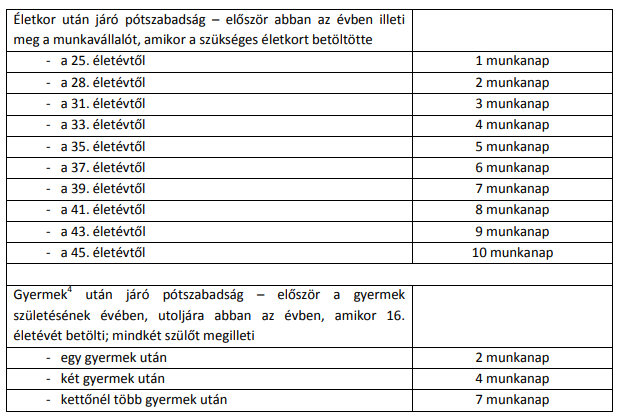
\includegraphics[scale=0.8]{images/potszabadsagok_1.png}
	\caption{Pótszabadságok típusai és értékei}
	\label{fig:potszab1}
\end{figure}

\begin{figure}[h]
	\centering
	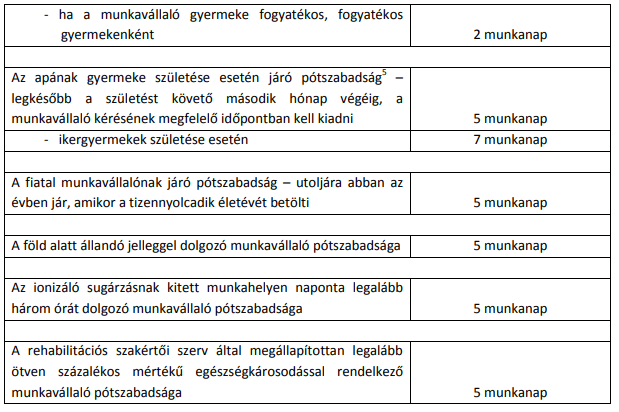
\includegraphics[scale= 0.8]{images/potszabadsagok_2.png}
	\caption{Pótszabadságok típusai és értékei}
	\label{fig:potszab2}
\end{figure}

\subsection{Közalkalmazottak szabadsága}

A közalkalmazottak szabadságolása nagyban eltér az átlag munkavállaló szabadságolásától. Alap szabadságuk fizetési osztálytól függően változhat, valamint nem teljesen ugyan azok a pótszabadságokkal kapcsolatos szabályok vonatkoznak rájuk mint egy átlag munkavállalóra.

"A közalkalmazottat
\begin{itemize}
	\item az „A”, „B”, „C” és „D” fizetési osztályban évi húsz munkanap,
	\item az „E”, „F”, „G”, „H”, „I”, „J” fizetési osztályban és a 79/C. §-ban említett munkakör betöltése esetén évi huszonegy munkanap
\end{itemize}

alapszabadság illeti meg."\cite{kozalkalmazottiSzabadsag}

\subsection{Időarányos szabadság}

"A munkavállalót a szabadság naptári évenként (tárgyév) illeti meg, ezért a részére járó szabadságnapok számát minden tárgyévben meg kell állapítani. Az ennek megfelelően meghatározott szabadság a munkavállalónak, ha munkajogviszonya a tárgyévben egészében nem áll fenn, azaz a naptári év közben létesül vagy szűnik meg, arányosan jár. " \cite{idoaranyosszabadsag}

Az éves szabadság megállapításakor tehát figyelembe kell vennünk, hogy a munkavállaló az adott évben ténylegesen mennyi munkanapot tölt alkalmazásban. Egy egyszerű matematikai képlet alkalmazásával számoljuk ki az alkalmazott éves szabadságát. 

Egy példán keresztül bemutatva a következőképp számoljuk egy munkavállaló időarányos szabadnapjait egy évre.

"A munkavállalót alapszabadságként 20 munkanap szabadság illeti meg naptári évenként. Ezen túlmenően az Mt. számos jogcímen (életkor alapján, 16 éven aluli gyermekekre tekintettel, speciális munkakörökben stb.) határoz meg pótszabadságokat, amelyek együttesen is megillethetik a munkavállalókat.

Az időarányosítás elvégzéséhez első lépésben meg kell állapítani a munkavállalót megillető szabadság mértékét. Ezt attól függetlenül munkanapban kell megtenni, hogy a munkáltató a szabadságot egyébként munkanapban vagy órában tartja nyilván.  Így például, egy harminchárom éves, két tizenhat év alatti gyermeket nevelő munkavállalót, aki állandó jelleggel föld alatt dolgozik, az alábbi jogcímeken illeti meg szabadság:

\begin{itemize}
	\item alapszabadság (20 munkanap)
	\item életkori pótszabadság (4 munkanap)
	\item gyermekek után járó pótszabadság (4 munkanap)
	\item föld alatti munkavégzés miatt (5 munkanap).
	\item föld alatti munkavégzés miatt (5 munkanap).
\end{itemize}

Azaz, a munkavállalónak mindösszesen 33 munkanap szabadsága van.

Az így megállapított összes szabadságot arányosítani kell, a munkaviszony év közben történő keletkezése, illetve megszűnése esetén. A fenti példában szereplő munkavállalót, amennyiben munkaviszonya 2016. július 1-jén fog elkezdődni (ekkor tárgyévben legfeljebb 184 napot fog munkaviszonyban állni) \( 33/365*184= 16,64 \) munkanap szabadság illetné meg.

Tekintettel arra, hogy az így kiszámított szabadság töredéknapot eredményez, alkalmazni kell az Mt. azon szabályát, hogy a fél napot elérő töredéknap egész napnak számít. Azaz, a munkavállalót mindösszesen 17 munkanap szabadság illeti meg 2016-ban."\cite{idoranyosSzamolasPelda}

Tehát az általános egyenlet a következő:
\begin{equation}\label{szabadság Számítás Tört Év esetén}
		\frac{MunkavallaloEvesSzabadsaga}{TargyEvNapokban*TargyEvbenHatralevoMunkanapok}=\lceil szabadsag \rceil
\end{equation}

\subsection{Szabadságok felhasználása}

Fontos tudni, hogy a munkavállaló nem rendelkezik teljes mértékben a számára meghatározott éves szabadság kerettel.

"A munkáltató évente hét munkanap szabadságot legfeljebb két részletben a munkavállaló kérésének megfelelő időpontban köteles kiadni azzal, hogy a munkavállalónak erre vonatkozó igényét legalább tizenöt nappal a szabadság kezdete előtt be kell jelentenie. A hét napos szabály jelentősége, hogy amennyiben a munkavállaló szabályszerűen bejelentette szabadságigényét, azt a munkáltató nem mérlegelheti.

Fontos, hogy ez a hét napos szabály a munkaviszony első három hónapjában nem köti a munkáltatót, azaz a munkaviszony első három hónapjában a munkavállaló a hét szabadnap általa meghatározott időpontban történő felhasználási jogával nem élhet. Ez utóbbi szabályt a legtöbbször – tévesen – úgy értelmezik, hogy próbaidő alatt, illetve az első három hónapban nem lehet szabadságra menni. [...]

Fontos kötelezettsége a munkáltatónak, hogy a szabadságot úgy kell kiadnia, hogy a munkavállaló naptári évenként egy alkalommal, legalább tizennégy egybefüggő napra mentesüljön a munkavégzési és rendelkezésre állási kötelezettsége alól. Ettől a szabálytól azonban a felek eltérhetnek.

A tizennégy napos szabály tekintetében – a szabadságként kiadott napon túl – a heti pihenőnap (heti pihenőidő), a munkaszüneti nap és az egyenlőtlen munkaidő-beosztás szerinti szabadnap vehető figyelembe." \cite{szabadsagFelhasznalasa}

\Section{Jelenleg elérhető megoldások}

A rengeteg szabályozásból, csak párat kiemelve jól látszik, hogy az automatizáláshoz szükséges számítások nem túl bonyolultak. A törvények összetett struktúrája, viszont országonként eltér, sőt a munkavállalókra különböző jogszabályok vonatkoznak amennyiben azok közalkalmazottak. Ezen információk fényében a vizsgálható, az elérhető megoldások amiket a jelenlegi piac kínál.

\subsection{Nemzetközi szoftverek}

Szinte számtalan applikáció elérhető a nemzetközi piacon, és ezek mindegyike minőségi szolgáltatás nyújt egy modern és könnyen kezelhető design keretében. Összességében mindegyikről elmondható, hogy ezek a szolgáltatások havidíjas előfizetéssel, működnek és többnyire tartozik hozzájuk egy profi támogatói csoport is akik mind konfigurálás, mind felhasználói problémák esetén is elérhetőek. 

Továbbá az is jól látszik, hogy több országban jelen vannak így nem csak az általános pótszabadságokat tudjuk ezeken keresztül kezelni, de akár saját személyre szabott típust is definiálhatunk.

Hátrányuk, viszont nem csak a havi díjban megszabott ár hanem az ehhez tartozó felhasználói létszám keret vagy akár a csomagban definiált funkció korlátozás is. Látható még, hogy ezek az alkalmazások vagy csak egy funkcióként kezelik a szabadság nyilvántartást, vagy egy több szolgáltatásból álló egység külön része ami arra enged következtetni, hogy bár külön álló program ként is funkcionál, bizonyos előnyök csak a többi testvér szolgáltatással együtt használhatóak.

Végül láthatjuk, hogy egyik alkalmazás bemutató anyaga sem tér ki a közalkalmazottakra, így azt feltételezhetjük, hogy ezek a szolgáltatások nincsenek felkészítve a közalkalmazotti különbségekre.

A \ref{tab:nemzetközi programok} \texttt{Nemzetközi programok összehasonlítása} táblázatban látható néhány elérhető megoldás.

\begin{table}[h]
	\centering
	\caption{Nemzetközi programok összehasonlítása.}
	\label{tab:nemzetközi programok}
	\begin{tabular}{|>{\centering\arraybackslash}m{3cm}|>{\centering\arraybackslash}m{5.5cm}|>{\centering\arraybackslash}m{5.5cm}|}
		\hline
		Termék megnevezése & Tulajdonságok & Csomag árak \\
		\hline
		freshworks, freshteam, Time Off\cite{freshworkswebsite} & Teljes körű HR szolgáltatás, felhasználó adatbázis, munkaidő követés, alapvető vagy akár bonyolult szabadság kezelés   & Ingyenes(nem tartalmaz egyéni szabadság kezelési lehetőséget), 75\$ - 250\$/hó/50 felhasználó \\
		\hline
		Leave Dates\cite{leavedateswebsite} & Idő menedzsment, szabadság kezelés  & Ingyenes 5 felhasználóig, 1\$/hó \\
		\hline
		AnnualLeave\cite{annualleavewebsite} & Idő menedzsment, szabadság kezelés  & Árajánlat kérés alapján, elérhető kalkulátoruk szerint 22\$/hó(20 főre) \\
		\hline
		Calamari\cite{calamariwebsite} & Szabadság kezelés, felső vezetői jóváhagyási rendszer, nemzetközi naptárak  & Felhasználók mennyiségétől függ 25\$/hó(20 főre) \\
		\hline
	\end{tabular}
\end{table}

\subsection{Magyar fejlesztésű programok}

A piacon található Magyar eredetű megoldások többsége valamiért még mindig az összetett excel táblázatokon alapul, amikben bonyolult függvények és macro programozással valósítják meg a nyomon követést.

Ezeknek a megoldásoknak a legnagyobb hibája a nehezen megoldható konkurens kezelés valamint, a felhasználó számítógépével való szoros függőség. Mindezek mellett sérülékeny, az óvatlan szerkesztés és mentés esetén könnyen az egész táblázat hamis adatokat mutathat. Esetleges hiba bekövetkeztével a pótlásuk nehézkes, szinte lehetetlen.

Fellelhetőek itt is kifejezetten a témával kapcsolatos szoftverek vagy akár teljes szolgáltatások is. Ezek a lehetőségek többnyire komplex rendszerek több, esetenként akár felesleges funkcióval.

A \aref{tab:magyar programok} \texttt{Magyar megoldások összehasonlítása} táblázatban látható néhány elérhető megoldás.

\begin{table}[h]
	\centering
	\caption{Magyar megoldások összehasonlítása}
	\label{tab:magyar programok}
	\begin{tabular}{|>{\centering\arraybackslash}m{3cm}|>{\centering\arraybackslash}m{5.5cm}|>{\centering\arraybackslash}m{5.5cm}|}
		\hline
		Termék megnevezése & Tulajdonságok & Csomag árak \\
		\hline
		Szabadság tervező és nyilvántartó\cite{hatekonysagwebsite} & Szabadság nyilvántartó excel táblázat   & 6 felhasználóig ingyenes, 21-50 felhasználóig 21.000 Ft + ÁFA/hó \\
		\hline
		excelmester\cite{excelmestergwebsite} & Szabadság nyilvántartó excel táblázat  & Ingyenes\\
		\hline
		HRmaster\cite{hrmasterwebsite} & Összetett erőforrás menedzser szoftver  & Árajánlat kérés alapján \\
		\hline
		PREDOR\cite{predorwebsite} & Munkaidő nyilvántartó és biztonsági rendszer  & Árajánlat kérés alapján \\
		\hline
	\end{tabular}
\end{table}

\Section{Fejlesztési lehetőségek}

Az elérhető megoldásokat összegezve láthatjuk, hogy többségük a munkavállaló szempontjából könnyen használható, mégis számunkra kényelmetlen konfigurációs problémákat vethet fel, amennyiben alkalmazottainkra eltérő szabályokat kell alkalmaznunk. Megfigyelhetjük azt is, hogy az összetettebb statisztikai lehetőségeket biztosító alkalmazások meglehetősen költségesek egy felsőoktatási intézmény számára, és akár megannyi számunkra kevésbé hasznos később kihasználatlan funkciót is tartalmazhatnak.

Továbbá általánosan elmondható a promóciós anyagok alapján, hogy az automatizált működés nincs megvalósítva.
\vskip 0.2in
Amennyiben leszűkítjük a felhasználók körét a felsőoktatásban dolgozó oktatókra és az azokkal együtt, tevékenykedő adminisztrátorokra láthatóvá válik, hogy bár az egyetemek használnak központi alkalmazásokat de egy-egy intézetben már megjelennek az eltérő szabályok. Egy egységben egyszerre vannak jelen normál, és közalkalmazotti jogviszonnyal rendelkező munkavállalók is, ezen felül szervezeti egységenként az-az tanszékenként, intézetenként a szabadságok jóváhagyásáért az adott egység vezetője a felelős. Felelősségi körébe viszont beletartozik egy éves szabadságolási terv előállítása is amelynek be kell tartania a szabadság felhasználásával kapcsolatos jogszabályokat is. Az említett tervezetet valamint időközi statisztikákat jelenleg manuálisan állítják össze és továbbítják a központi rendszerbe.
\vskip 0.2in
Mindent egybevetve a piacon fellelhető applikációk több extra funkciótól mentes de mégis számunkra specifikus alkalmazást hozhatunk létre a következő működések megvalósításával:

\begin{itemize}
	\item A felhasználó egyedi szabadságolással kapcsolatos adatait tartalmazó adatbázis
	\item A Magyar törvényekre specifikus szabadság típusoknak megfelelő konfigurálási lehetőség
	\item Dinamikus alkalmazhatóság, eltérő alkalmazotti jogkörök esetén.
	\item Automatikus kalkuláció teljes és részleges tárgy év esetén.
	\item Felettesi jóváhagyás támogatása.
	\item Éves szabadságolási tervező / Automatikus generálás.
	\item Tetszőleges statisztikák lekérdezése.
	\item Felhasználó jól átlátható, követhető szabadnap menedzsmentje.
\end{itemize}

\Section{Technológiai eszköztár}

A konkrét tervezési lépések megkezdése előtt rendkívül fontos az alkalmazásunk számára megfelelő technológiai hátteret biztosítani.

Választásunk során nem elég figyelembe venni mi az amit kezelni tudunk, fontos előretekintően lehetőleg minél modernebb technológiákat alkalmazni amik nagyban könnyíthetik bizonyos műveletek elvégzését a megvalósítás során, valamint lehetőséget nyújtanak a későbbi fejlesztés egyszerűsítésére is.

Ellenben nem érdemes kiforratlan kezdetleges de divatos eszközökhöz sem, hozzákötni magunkat!

\subsection{Verziókezelés és Verziókezelő rendszerek}

"Verziókezelés alatt több verzióval rendelkező adatok kezelését értjük. Leggyakrabban a mérnöki tudományokban és a szoftverfejlesztésben használnak verziókezelő rendszereket fejlesztés alatt álló dokumentumok, tervek, forráskódok és egyéb olyan adatok verzióinak kezelésére, amelyeken több ember dolgozik egyidejűleg. Az egyes változtatásokat verziószámokkal vagy verzióbetűkkel követik nyomon."\cite{verziokezeles}

Lényeges pontja a fejlesztésnek, hogy a forráskód, ne csak a saját gépünkön legyen elérhető, amennyiben csapatban dolgozunk ez a szempont kiemelten fontos lehet, nagyban könnyítheti a mindennapokat, ha egymástól függetlenül könnyen tudunk változtatásokat eszközölni a kódbázison.

Ezeknek a rendszereknek a gyakorlati haszna túlmutat a forráskód konkurens kezelhetőségén, stabil verziók esetén szerves részét képezik mindennapi használatban lévő úgynevezett "éles" vagy "production" környezetbe való kitelepítését.

\paragraph{SVN}

"A Subversion (SVN) egy verziókezelő rendszer, melyet a CollabNet Inc. indított 2000-ben. Fájlok aktuális verzióinak és történeteinek kezelésére használják, mint például forráskódok, weboldalak és dokumentációk. A célja, hogy a legkompatibilisebb utódja legyen a széles körben használt Concurrent Versions System (CVS)-nek."\cite{svn}

Az SVN alapú rendszerek jól használhatóak a lineáris fejlesztésben, de agilis fejlesztési modell esetén sokkal nem elég rugalmasak és nehezebben kezelhetőek.

Korábban a legnépszerűbb használatban lévő rendszer, mai napig megtalálható a piacon, viszont a modernebb koncepciók elterjedésével egyre ritkábban találkozhatunk SVN-ben kezelt kódbázissal.

\paragraph{Git}

"A Git egy nyílt forráskódú, elosztott verziókezelő szoftver, vagy másképpen egy szoftverforráskód-kezelő rendszer, amely a sebességre helyezi a hangsúlyt. A Gitet eredetileg Linus Torvalds fejlesztette ki a Linux kernel fejlesztéséhez. Minden Git munkamásolat egy teljes értékű repository teljes verziótörténettel és teljes revíziókövetési lehetőséggel, amely nem függ a hálózat elérésétől vagy központi szervertől."\cite{git}

Gyors és skálázható rendszer, könnyen és dinamikusan kezelhető kis és nagy létszámú csapatok esetén is. Gyorsan tanulható és könnyen átlátható, a lokális repository már kezdő fejlesztőként is segíti és gyorsítja az egyes fejlesztési műveleteket. Megfelelő beállítások, használat esetén a központi repository stabil ága jól védett, ezáltal folyamatos lehetőséget biztosít az általunk fejlesztett szoftver legfrissebb működő állapotának az "éles" végfelhasználók számára elérhető környezetre való kitelepítését.

Jelenleg széles-körben használt, elterjedt és népszerű technológia. A megvalósítás során én is ezt a technológiát használtam fel.

\subsection{Programozási nyelvek}

Webfejlesztés esetén több meghatározó területet definiálhatunk, de ezek közül is leginkább a Backend az-az háttér rendszeri fejlesztés, valamint a Frontend tehát a felhasználói felület és megjelenítés fejlesztés amit főbb tagolásnak nevezhetünk. Ezek a területek funkciójukban és feladatkörükben elválaszthatóak, többnyire külön micro alkalmazások ként működnek, így fontos megemlíteni, hogy bár minden esetben egymással kommunikálnak, többnyire egymástól független programozási nyelveken íródnak.

Mind a két területről elmondható, hogy nagy választékkal rendelkeznek nyelvek területén, ezek folyamatosan megújuló megoldások ezért ezen a területen kiemelten fontos, hogy körültekintően válasszunk! Egy friss és dinamikus megoldásokat kínáló nyelv gyakran lehet kiforratlan és kevésbé előnyös a későbbi fejlesztések során a jól bevált már ismert nyelvekkel szemben.

\paragraph{Háttérrendszer, Backend}

Ezen a területen bár mostanában kezd elterjedni a node.js, mégis a C\# és Java nyelveket mondhatjuk meghatározónak. Bár mind a C\# is elismert és több helyen használt, mégis mondhatni jelenleg a Webfejlesztés piacán a Java az elterjedtebb és támogatottabb nyelv.

\subparagraph{Java}

"A Java általános célú, objektumorientált programozási nyelv, amelyet a Sun Microsystems fejlesztett a ’90-es évek elejétől kezdve egészen 2009-ig, amikor a céget felvásárolta az Oracle.

A Java alkalmazásokat jellemzően bájtkód formátumra alakítják, de közvetlenül natív (gépi) kód is készíthető Java forráskódból. A bájtkód futtatása a Java virtuális géppel történik, ami vagy interpretálja a bájtkódot, vagy natív gépi kódot készít belőle, és azt futtatja az adott operációs rendszeren. Létezik közvetlenül Java bájtkódot futtató hardver is, az úgynevezett Java processzor.

A Java nyelv a szintaxisát főleg a C és a C++ nyelvektől örökölte, viszont sokkal egyszerűbb objektummodellel rendelkezik, mint a C++. A JavaScript szintaxisa és neve hasonló ugyan a Java-hoz, de a két nyelv nem áll olyan szoros rokonságban, mint azt ezekből a hasonlóságokból gondolhatnánk. [...]

A nyelv első tulajdonsága, az objektumorientáltság („OO”), a programozási stílusra és a nyelv struktúrájára utal. Az OO fontos szempontja, hogy a szoftvert „dolgok” (objektumok) alapján csoportosítja, nem az elvégzett feladatok a fő szempont. Ennek alapja, hogy az előbbi sokkal kevesebbet változik, mint az utóbbi, így az objektumok (az adatokat tartalmazó entitások) jobb alapot biztosítanak egy szoftverrendszer megtervezéséhez. A cél az volt, hogy nagy fejlesztési projekteket könnyebben lehessen kezelni, így csökken az elhibázott projektek száma. [...]

A Java legfontosabb része a Java virtuális gép (Java Virtual Machine – JVM). A JVM mindenütt jelen van (szinte mindenféle berendezés, chip és szoftvercsomag tartalmazza), így a nyelv középszintként és platformként egyaránt működik. Ugyanakkor a nyelv „platformfüggetlen” is, mert a Java virtuális gépek interpretálják a szabványos Java bájtkódot. Ez azt jelenti, hogy egy PC-n megírt Java program minimális módosítás után ugyanúgy fog futni egy javás telefonon is. Innen jön az írd meg egyszer, futtasd bárhol kifejezés. Ez jelentős költségcsökkenést eredményez, mert a kódot csak egyszer kell megírni."\cite{java}

A megvalósítás során Java 11-es verziót használtam, melyben elérhetőek a lambda és stream nyelvi elemek.

\paragraph{Megjelenítés, Frontend}

A megjelenítési réteg webapplikációk esetén többnyire három fő részből áll. A HTML leírónyelveben íródó struktúra adja az oldalak felépítését, vázát. Ezt kiegészíti egy másik leíró nyelv a CSS ami minden esetben a megjelenő designért felelős. Valamint ide tartoznak még a különböző script nyelvek mint a javascript amelyek az böngészőben futó logikáért felelősek.
\vskip 0.2in
Java nyelv esetén beszélhetünk még a JSP technológiáról ami az említett frontend technológiákat ötvözte valamint lehetővé tette, hogy Java kódot építsünk be HTML-be. Ezzel elértük, hogy az alkalmazásunk szerves része legyen egy általunk generált megjelenés is. 

A mára elavultnak számító JSP technológiát egyszerűbb esetekben a hasonló működési elven alapuló szerver oldalon generált megjelenést biztosító Java template engine-ek váltották fel több helyen. Használatukban igen hasonlóak az elődjükhöz, viszont a különböző Java logikák mint az if vagy a for használata sokkal egyszerűbb és átláthatóbb. Az egyik legnépszerűbb alkalmazás ezen a téren a Thymleaf. 

\vskip 0.2in
A legmodernebb megoldás jelenleg az Angular logikával megvalósított megjelenítés. Ezen esetben is jelen van a HTML, valamint a CSS viszont az oldalunk tartalmát és akár megjelenítését is tudjuk változtatni akár csak a sima javascript esetén. Ez az elképzelés viszont objectum orientált alapokra helyezi a frontend fejlesztést, valamint saját különálló programként tekint a megjelenítési réteg kódbázisára. 

Tehát ebben az esetben arról beszélhetünk, hogy önállóan is futtatható a programunk megjelenítési rétege, így az a hátétrendszertől elkülönítve fejleszthető a két alkalmazás. Csupán kommunikációs kapcsolat van köztük így amennyiben arra igény van a megjelenítés, valamint a szerver oldali logika egymástól függetlenül cserélhető is.

\vskip 0.2in
Itt érdemes még megemlíteni az előre definiált designt biztosító Bootstrap szolgáltatást is, ami lehetővé teszi, hogy a megjelenítést gyorsan felépítsük már létező CSS elemekkel.

\subsection{Szoftver menedzsment eszköz}

Mivel meglehetősen időigényes akár a mindennapi fejlesztés terén az alkalmazásunk futtatására különféle parancsok megfelelő sorozatát kiadni, így igény keletkezett az automatizálható szoftver menedzsment eszközökre. Az egyik ilyen legelterjedtebb az Apache Ant volt eleinte. Viszont mára sokkal ismertebb és elterjedtebb a szintén Apache fejlesztésű Maven használata.

\paragraph{Maven} "Az Apache Maven (röviden Maven) egy szoftver, amelyet szoftverprojektek menedzselésére és a build folyamat automatizálására lehet használni. Jason van Zyl készítette 2002-ben. Funkcionalitásában hasonlít az Apache Ant eszközhöz (és némi hasonlóságot mutat a PHP-s PEAR-rel és a perles CPAN-nal, de egyszerűbb és XML-alapú a konfigurációs modellje). A projektet az Apache Software Foundation hosztolja, ahol korábban a Jakarta Projekt részeként működött.

A Maven bevezeti a POM, azaz a Projekt Objektummodell (angolul: Project Object Model) fogalmát. Egy POM egy buildelendő projektet ír le és annak függőségeit. Az egyes lépéseket céloknak, angolul goal-oknak nevezik. Vannak előre definiált célok a tipikus feladatokra, mint például a kód fordítása és csomagolása, de a felhasználónak lehetősége van saját célokat is definiálni a projektspecifikus lépések végrehajtására.

A Maven hálózatképes, tehát szükség esetén dinamikusan is le tud tölteni komponenseket. Repository névvel illetik a különböző hosztok fájlrendszereinek azon mappáit, ahol a letölthető komponensek találhatók. A Maven nem csak a repository-kból való letöltést támogatja, hanem a készült szoftvercsomag feltöltését is. Ezzel az automatizálható le- és feltöltési mechanizmussal a Maven de facto szabványt próbál teremteni, de elég lassan fogadja el a Java közösség.

A Maven plugin alapú architektúrája lehetővé teszi tetszőleges parancssorból vezérelhető alkalmazás használatát. Ez elméletileg lehetővé teszi tetszőleges programnyelvekhez való pluginek készítését, de a gyakorlatban minimális mennyiségű nem javás plugin készült."\cite{maven}

\vskip 0.2in
Fontos megemlíteni, hogy bár a Maven jelenleg a legelterjedtebb manapság egyre népszerűbb a Gradle is, ami átláthatóbb és dinamikusabban konfigurálható, mégis egyetlen hátránya van ami miatt kevesebben használják és ez csupán az, hogy kevésbé ismert.

\subsection{Keretrendszerek}

Habár csak és kizárólag Java nyelv használatával is képesek vagyunk megvalósítani egy számunkra megfelelő alkalmazást, mégis érdemes megkönnyíteni a saját dolgunkat különböző keretrendszerek használatával. Korábban ilyen volt a Java EJB, mára viszont sokkal kifinomultabb megoldások léteznek, a webalkalmazások terén az egyik legismertebb a Spring valamint az arra épülő Spring-boot.

\paragraph{Spring}

"A Spring egy nyílt forráskódú, inversion of controlt megvalósító Java alkalmazás keretrendszer.
A Spring keretrendszer több önálló modulból épül fel, amelyek az alábbi szolgáltatásokat nyújtják a fejlesztők számára:

\begin{itemize}
	\item Inversion of control konténer: a Java objektumok életciklusának kezelése és az alkalmazás-komponensek testreszabása.
	\item Aspektus orientált programozási paradigma követésének lehetősége.
	\item Adatelérés: lehetőség van relációs adatbázis-kezelő rendszerek JDBC segítségével történő elérésre, és objektum-relációs leképzések, NoSQL integrálására.
	\item Tranzakciókezelés: többféle tranzakció kezelő API-t tartalmaz.
	\item Modell-nézet-vezérlő szabvány: egy HTTP- és servlet alapú keretrendszer segítségével valósítható meg, amelyet arra fejlesztettek ki, hogy bővíthetők és személyre szabhatóak legyenek a webszolgáltatások
	\item Távoli eljáráshívás kezelő keretrendszer: biztosítja a RPC alapú, hálózaton keresztül történő Java objektum importokat és exportokat. További támogatást nyújt a RMI, a CORBA és HTTP alapú protokollok \item használatára, beleértve a webszolgáltatásokat (SOAP) is.
	\item Kötegelési eljárás támogatása.
	\item Azonosítás és azonosságkezelés: biztonsági folyamatok konfigurálása, melyet a Spring projekthez tartozó, Spring Security alprojekt tesz lehetővé a különféle protokollok és módszerek biztosításával.
	\item Üzenetkezelés: a JMS API-n keresztül történő általános üzenetkezelés továbbfejlesztése érhető el.
	\item Tesztelés: segítséget nyújt a unit- és az integrációs teszt írására."\cite{spring}
\end{itemize}

\subparagraph{Inversion of control (IoC) avagy a kontroll megfordítása} "főleg objektumorientált programozási nyelvekben használt technika a komponensek összeillesztésére, konfigurálására és kezelésére.

A technika lényege, hogy a komponenskezelést (pl. létrehozást, példányosítást, paraméterezést, megszüntetést, metódus hívás) kiemeljük a programkódból, és általában egy külső keretrendszerre bízzuk, mint pl. a Spring.

Célja a modularitás növelése és bővíthetővé tétele. Az objektumorientáltság nem feltétel. A kifejezést Robert C. Martin és Martin Fowler népszerűsítette.

Egy rokon minta a függőség befecskendezése, ami a függőségeket megosztott absztrakcióval kezeli a felső és az alsó rétegek között. Kapcsolódik az eseményvezérelt programozáshoz is, mert azt gyakran a kontroll megfordításával valósítják meg. A felhasználó kódja csak az eseményeket dolgozza fel, míg az eseményciklus és az események, üzenetek közvetítése a keretrendszerre vagy a futtató környezetre van bízva."\cite{ioc}

\subparagraph{Spring konfigurálása}

Ahhoz, hogy az általunk megírt osztály a keretrendszerben létezzen, konfigurálnunk kell belőle egy példányt amit fel tud dolgozni és a saját kontextusába be tud illeszteni. Ennek az úgynevezett bean definíciónak három módja van. XML, Java valamint annotáció alapú konfigurációból választhatunk, de akár keverhetjük is őket ami nehezíti a kód megértését így semmiféleképp nem ajánlott. Mindegyiknek megvan természetesen a maga előnye és hátránya. Csak rajtunk múlik melyiket használjuk de fontos, hogy lehetőleg maradjunk egy félénél és legyen konzisztens a kódunk.

\paragraph{Spring-boot}

Egy natív Spring alapú szolgáltatás melynek lényege, hogy gyorsan és még egyszerűbben tudjunk önálló webalkalmazásokat létrehozni. Amíg az egyszerű Spring esetén az összes elemet nekünk kell összerakni és bekonfigurálni, a boot esetén előre definiált egységeket használunk ami egy kezdetleges konfigurációval rögtön futtatható programot biztosít számunkra.

Továbbá ezen külső könyvtárak és megvalósítások újra konfigurálása is sokkal egyszerűbb.

Tartalmaz előre meghatározott annotációkat amik használatával másodpercek alatt hozhatunk létre a keretrendszer kontextusában létező osztályokat.  

\subsection{Adatbázis, Verzió kezelt adatbázis, ORM}

Napjainkban egyre több típusú adatbázis létezik, és mindegyiknek megvan a leghasznosabb felhasználási területe, már nem csak a jól ismert SQL típusok érhetőek el de megjelent a NoSQL valamint sok más koncepció alapján működő lehetőség is.

A megvalósítás szempontjából szinte tökéletesen megfelel a mindenki által ismert SQL típus, ez egy igen széles-körben elterjedt és alkalmazott adatbázis.

\paragraph{Liquibase} "egy ingyenes, nyílt forráskódú, adatbázisfüggetlen változáskövető eszköz, ami jól használható az elterjedt verziókövető eszközökkel. Lényege, hogy a szükséges adatbázismódosításokat nem közvetlenül az adatbázison hajtjuk végre, hanem minden változást struktúrált módon, egy ún. changelog fájlban tartunk nyilván. Ezt a changelog fájlt aztán a Liquibase parancssoros alkalmazás segítségével vagy kódból, a Liquibase Java API-val tudjuk érvényesíteni. Ennek használata a következő előnyökkel jár:

\begin{itemize}
	\item a changelog fájl feltölthető verziókövetőbe, ezáltal megvalósíthatjuk adatbázisunk verziókövetését;
	\item a Liquibase számon tartja, hogy mely változások kerültek korábban már érvényesítésre adatbázisunkon, és csak a szükségeseket futtatja." \cite{liquibase}
\end{itemize}

\paragraph{Objektum-relációs leképzés(ORM)}
"Az objektum-relációs leképzés (angolul \newline Object-Relational Mapping) egy programozási technika adatok konvertálására nem kompatibilis típusos rendszerek és objektumorientált programozási nyelvek között. Lényegében egy „virtuális objektum-adatbázist” hoz létre, amit a programozási nyelvben használhatunk."\cite{orm}

Egyik legismertebb megvalósítása a JPA, ami nem csak a részét képezi a spring-bootnak, hanem saját ORM rendszert épít rá Spring Data néven.

\subsection{Szoftver architektúra}

"A modell-nézet-vezérlő (MNV) (angolul model-view-controller) a szoftvertervezésben használatos programtervezési minta. Összetett, sok adatot a felhasználó elé táró számítógépes alkalmazásokban gyakori fejlesztői kívánalom az adathoz (modell) és a felhasználói felülethez (nézet) tartozó dolgok szétválasztása, hogy a felhasználói felület ne befolyásolja az adatkezelést, és az adatok átszervezhetők legyenek a felhasználói felület változtatása nélkül. A modell-nézet-vezérlő ezt úgy éri el, hogy elkülöníti az adatok elérését és az üzleti logikát az adatok megjelenítésétől és a felhasználói interakciótól egy közbülső összetevő, a vezérlő bevezetésével.

Hagyományosan asztali felhasználói felületekhez használt, de manapság már webalkalmazásokhoz is népszerűvé vált. Népszerű programozási nyelvek mint a JavaScript, Python, Ruby, PHP, Java, C\# és Swift már külön telepítés szükségessége nélkül rendelkeznek MNV keretrendszerekkel web- és mobilalkalmazások fejlesztésére."\cite{mvc}

\begin{figure}[h]
	\centering
	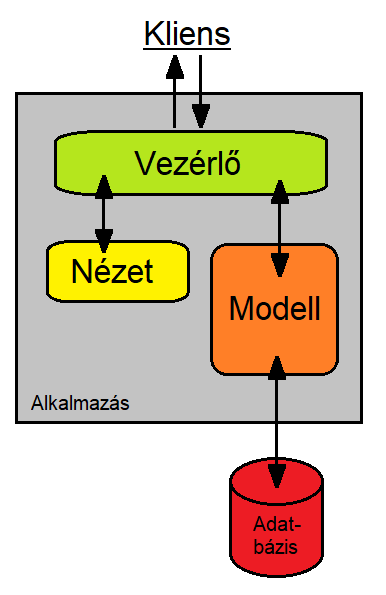
\includegraphics[scale= 0.8]{images/MNV-reprezentáció.png}
	\caption{MNV reprezentációja}
	\label{fig:mnv}
\end{figure}

Az MNV egy összetettebb változata  a több szintű architektúra amiben a korábban említett három rétegen felül saját rétegeket definiálunk és azok között belső transzformációkkal továbbítjuk az adatokat. Ilyen további rétegek lehetnek az Adat továbbítóréteg(DTO), a tartomány réteg (Domain) valamint az adat hozzáférési réteg (dal).

\vskip 0.2in
A többszintű alkalmazás architektúrák könnyebben átalakíthatóak Microservice architektúrákká, melyek fejlesztése és üzemeltetése egyszerűbb, költséghatékonyabb és stabilabb. 

\subsection{Tesztelés, Tiszta kód}

A fejlesztési folyamatok során elengedhetetlen, hogy folyamatosan kipróbáljuk és ellenőrizzük az általunk írt logikát. Ezeket az ellenőrzési folyamatokat nevezzük tesztelésnek.

A felületen történő funkcionális teszttől egészen a legapróbb kódsorig rengeteg lehetőségünk van a programunkat különböző tesztek alá vetni, hogy ténylegesen az elvárt működésnek megfelelően viselkedjen a szoftverünk.
Ezekhez támogatást nyújt számunkra a már említett Maven, valamint a Spring keretrendszer is. 

Különböző tesztelést segítő megoldások léteznek ilyen például a JUnit4, JUnit5 valamint a TestNG is, hogy  megtudjuk határozni a tesztek hatáskörét és garantáljuk egymástól való függetlenségüket, valamint, hogy meghatározzuk külső függőségek visszatérési értékét objectum utánzó objectumokat más néven Mock-okat használunk.

\paragraph{Egységtesztelés} "A számítógép-programozásban az egységtesztelés a szoftvertesztelésnek egy olyan módszere, amelynek során a forráskód egységeit (egy vagy több számítógépes program modul készletet) a kapcsolódó vezérlő adatokkal, a felhasználási-és a működtető eljárásokkal együtt tesztelik annak meghatározására, hogy azok elérik-e kitűzött céljukat."\cite{unittest}

Egység tesztelés során fontos meghatároznunk, mi az a legkisebb egység amit tesztelünk, általános megállapodás szokott lenni, hogy egy függvényt tekintünk tesztelendő egységnek. További megállapodás, hogy csak publikus elérésű függvényekre írunk tesztet, viszont a vélemények sokszor eltérnek a tesztesetek számát illetően. Vannak nézetek ami szerint minden lehetséges esetet le kell fedni, de a gyakorlatban legtöbbször csak az elvárt működést valamint a logika különböző agait szokás lefedni.

\paragraph{Manuális tesztelés}

Ahhoz, hogy az elvárt működést teljesen le tudjuk ellenőrizni, működés közben teszt adatok segítségével úgymond felhasználóként kipróbáljuk a funkciókat a felületen keresztül. Amennyiben csak háttérrendszerrel rendelkezünk ez a tesztelés továbbra is alkalmazható, a korábban már tárgyalt MNV modell miatt. A vezérlőt közvetlenül meg tudjuk hívni szimulálva ezzel a megjelenítési rétegtől érkező kérést, a szerver oldali alkalmazás pedig kiszolgálja azt egy JSON válasszal.

Ennek vizualizációjára szolgál a swagger-UI vagy más neven OpenAPI eszköz.\footnote{A dolgozat későbbi részében részletes bemutatásra kerül.}

\subparagraph{Tiszta kód}

Fontos megemlíteni, hogy a tesztek olvashatósága és egyszerűsége érdekében jól tagolt olvasható kódot kell produkálnia a fejlesztőnek. Ehhez szükség van előre definiált mérőszámokra mint például sorok hossza, függvények sorszáma, ciklomatikus komplexitás.

A nehezen olvasható és tesztelhető kódok, nagyobb valószínűséggel tartalmaznak hibát és szinte biztos, hogy újraírásra szorulnak.

A tiszta kód szabályai mindig a fejlesztőcsoport megegyezése alapján történnek, a szabályok betartása viszont nagyban könnyíti a későbbi fejlesztést. A megalkotásukhoz kiváló útmutató Robert C. martin, Clean Code : A Handbook of Agile Software Craftsmanship\cite{cleanCode} című könyve!

\subsection{Folyamatos integráció/Folyamatos szállítás (CI/CD)}

"A folyamatos integráció olyan fejlesztési gyakorlat, amelyben a fejlesztők a kódot naponta többször egy közös felületen integrálják, egyeztetik. Így a kisebb változtatások is gyorsan elérhetővé válnak a csapat többi tagja számára. Az integrálást követően minden új kódrészlet ellenőrzésre kerül, amely lehetővé teszi a fejlesztők számára, hogy korán felismerjék a problémákat és még az elején javítsák azokat, így időt nyerve és minimalizálva a javítandó kódok mennyiségét.

A folyamatos szállítás a folyamatos integráció természetes kiterjesztése: olyan megközelítés, amelyben a csapatok biztosítják a rendszer gyors kiadhatóságát verziónként. A folyamatos szállítás célja, hogy minél előbb visszajelzést kapjunk a munkánkról, hogy azt minél tökéletesebben a megrendelő igényeihez igazíthassuk, és ezzel minél nagyobb elégedettséget érjünk el a megrendelőknél."\cite{CICD}

A folyamatos integráció automatizált működése egy központi szerveren úgynevezett futtatók segítségével elindítja a szoftver menedzsment eszközt, ami felépíti a az applikációt, futtatja az általunk megírt teszteket valamint képes statikus kód analízist is végezni amennyiben azt előre definiáltuk. Ezek az analízisek segítenek rákényszeríteni a programozót a fejlesztés során a tiszta kód szabályainak betartására is.

Amennyiben folyamatos integrációt és folyamatos szállítást alkalmazunk képesek vagyunk olyan konfigurációra ami a megfelelő munkafolyamatok sikeres futtatása esetén a csővezeték utolsó munkafolyamata ként automatikusan telepíti az applikációnk legújabb verzióját egy az általunk meghatározott szerverekre.\footnote{A dolgozat későbbi részében részletes bemutatásra kerül.}

\Section{A fejlesztéshez szükséges ismeretek összefoglalása}

Ez a fejezet először bemutatta azokat a szabályozásokat amik segítségével részletes betekintést nyerhetünk a Magyar szabadságolás rendszerébe és megismerhettük annak összetettségét. Ezután általános képet kaphattunk az elérhető szolgáltatások és applikációkról működéséről, előnyeiről és hátrányairól, valamint a felhasználói igényekről, a Magyar Felsőoktatás szemszögéből. Ezen lehetősége költséges és kompromisszumokkal teli szolgáltatás nyújtanának ezekben a komplex szervezeti egységekben. Ezáltal elmondhatjuk, hogy egy saját célszoftver létrehozása nagyban segíthetné a szervezet részegységeinek munkáját, az igények és szabályok ismeretében képesek vagyunk ezt az applikációt megtervezni és megvalósítani. Végezetül felépítettük a tervezéshez és megvalósításhoz szükséges technológiai eszköztárat ami a rendelkezésünkre áll, és segítségével kivitelezhető egy webapplikáció ami nem csak kiszolgálhatja a korábban definiált elvárásokat, de akár igény szerint tovább is fejleszthető.
  
\Chapter{Automatizálható Webapplikáció Tervezése}

A fejezet célja, hogy a korábban megismert fogalmak és elvárások segítségével, létrehozzunk egy alkalmazás csontvázat aminek az implementálásával egy jól strukturált könnyen karbantartható és fejleszthető megoldást valósíthassunk meg.

További fejlesztések esetén ezen dokumentáció alapján, akár új fejlesztők is betudjanak csatlakozni a megvalósításba.  

\Section{Architektúra felépítése}

\subsection{Több rétegű alkalmazás}
Az MNV ismertetése során felmerült már a Többrétegű alkalmazás architektúra, lényegében véve nem sokban különbözik egymástól a két rendszer struktúrája, csupán további rétegeket vezetünk be, annak érdekében, hogy alkalmazásunkban jobban elkülönítsük a rétegek szerepeit. Ebben a felépítésben viszonylag kötöttebb szabályok mentén kell haladnunk, de az adataink a rétegek közötti átalakítások miatt nagyobb biztonságban vannak.

Hátránya viszont, a kódsorok száma és a fejlesztési idő is jelentősen megnövekedhet az alkalmazásával.

A rendszer tervezett felépítése a \aref{fig:architektura}. ábrán látható, ahol megfigyelhetjük, hogyan halad végig a különböző rétegeken a felhasználói kérés. 

\vskip 0.2in
Az ábrán látható folyamat során a felhasználótól érkező adat feldolgozódik a megjelenítési rétegben, majd az általunk írt Angular applikáció egy JSON objektumot generál és egy HTTP híváson keresztül megszólítja a szerveren futó alkalmazást. 

\begin{figure}[h]
	\centering
	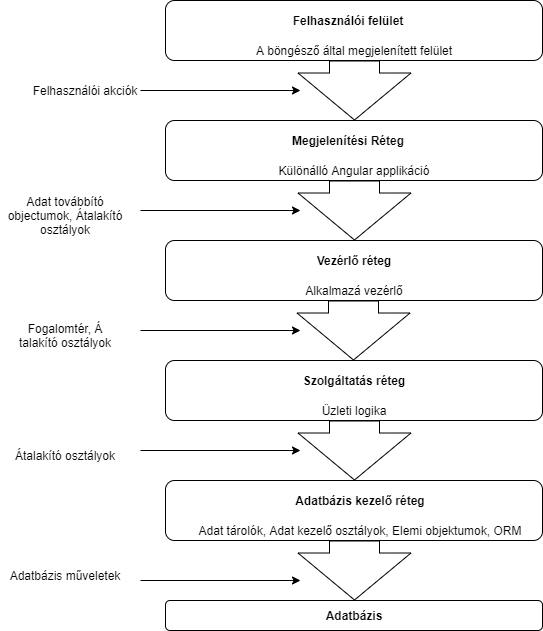
\includegraphics[scale=0.6]{images/applikacio_architektura.png}
	\caption{Többrétegű alkalmazás architektúra.}
	\label{fig:architektura}
\end{figure}

A háttérrendszer által definiált végponton a beérkező JSON kérést egy Adatközvetítő objektummá alakítjuk\footnote{Ennek az objektumtípusnak a fontosságát később kifejtem.}, ezt az objektumot átalakítva átadjuk a szolgáltatási rétegnek. 

Ebben a rétegben feldolgozzuk az adatokat, számításokat végzünk vele, majd a végső formájában átadjuk ismét egy átalakító osztálynak ahol Elemi objektummá alakítjuk.

Az adatkezelő rétegben, hozzáférünk az adatbázis kapcsolatainkhoz így az Elemi értékekből SQL-t létrehozva tudjuk meghívni az adatbázis egyes tábláit, ezzel beszúrni vagy akár lekérdezni adatokat azokból.

\subsection{Megjelenítési réteg}

Az alkalmazásunk itt rendereli ki a felhasználó számára látható és elérhető weboldalt, ez a művelet jól elkülöníthető, akár külön kódbázis és infrastruktúra is tartozhat hozzá, amennyiben nem a már említett JSP technológiát vagy sablon alapú megjelenítést használjuk.
\vskip 0.2in

Az Angulár használata mindenféleképp külön webszerver indítását igényli így érdemes ennek megfelelően különálló logikaként kezelni, akár egy önálló microalkalmazásként is tekinthetünk rá.

A programozási nyelv segítségével képesek vagyunk dinamikusan ellenőrizni a felhasználótól kapott bemeneti értékeket és nem megfelelő adat esetén rögtön jelezni az eltérést, ezzel segítve az elvárt működést.

Fontos, hogy a felhasználói felület letisztult és könnyen használható legyen, ugyanakkor az adatok kezelésében minden esetben a felület igazodik, a szerver oldali logikához. Nem itt definiáljuk az elküldött vagy elvárt JSON üzenetek tartalmát és felépítését. Több fejlesztő esetén a résztvevők közösen egyeznek meg az értékekről és a struktúráról.

\paragraph{Általános felület terv:} A könnyen kezelhetőséget szem előtt tartva a \aref{fig:felület_terv}. látható listanézetes megjelenítést érdemes használni az alkalmazás összes funkciójánál, hogy egyes adatokat megjelenítsünk.

Ennek a nézetnek a segítségével láthatóvá tesszük az elérhető adatokat, azokat az elhelyezett gombok segítségével szerkeszthetjük amik kattintás után az ehhez szükséges űrlaphoz navigálnak. Ezen az oldalon továbbá elérhetőnek kell lennie az elemi műveletekhez szükséges gomboknak mint például törlés, mentés.

\begin{figure}[h]
	\centering
	\includegraphics[scale=0.3]{images/felület.png}
	\caption{Általános felület terv}
	\label{fig:felület_terv}
\end{figure}

\footnote{A jogkörökről és azokhoz tartozó funkciókról a dolgozta későbbi részében lesz szó.}

Az általános felület mintájára a következő típusú felületek megvalósítása szükséges:

\begin{enumerate}
	\item Minden felhasználó számára elérhető.
	\begin{itemize}
		\item Saját adatok megtekintése.
		\item Felhasználható és felhasznált szabadnapok nyomon követése.
		\item Szabadnapok kiírása és módosítása.
	\end{itemize}
	\item Jóváhagyó számára elérhető.
	\begin{itemize}
		\item Vele relációban álló felhasználók szabadnapjainak nyomon követése.
		\item Jóváhagyásra váró kérések listája, azokhoz tartozó műveletek.
	\end{itemize}
	\item Adminisztrátor számára elérhető
	\begin{itemize}
		\item Szabadságolással kapcsolatos konfigurációs oldalak.
		\item Vele relációban álló felhasználók létrehozása, adatainak módosítása.
	\end{itemize}
\end{enumerate}

Továbbá az adminisztrátor és a jóváhagyó számára egy statisztikai összesítéseket megjelenítő oldal, valamint egy éves szabadságolási terv létrehozására és módosítására alkalmas naptár nézettel rendelkező oldal megvalósítására is szükség van.

\subsection{Vezérlő réteg, és Adatközvetítő objektumok}

Az alkalmazásunk szerver oldali megvalósítása a vezérlőrétegnél kezdődik, itt definiálhatjuk a végpontokat amik segítségével kommunikálhatunk a közvetlen felettünk lévő réteggel. Ezek a végpontok URL paraméterként jelennek meg, így könnyedén hivatkozhatunk rájuk.

\paragraph{Vezérlőfüggvények}
Minden függvényhez rendelünk egy URL értéket amin keresztül a függvény meghívódik, az argumentumaink attól függően változhatnak milyen HTTP hívásnak feleltetjük meg a függvényt. 

Elemi adattípusok esetén az URL paramétereként adjuk át a kívánt információt, objektumot viszont JSON kérésként kezelünk. Ahhoz, hogy a beérkező JSON értékből számunkra kezelhető objektum legyen szükségünk van egy Adatközvetítő objektumra. 

Ezek a függvények minden esetben átadják az adatot egy átalakító osztálynak ami egy Belső objektumot hoz létre és tovább adja azt a megfelelő szolgáltatás osztálynak.
\paragraph{Adatközvetítő objektumok}
Kifejezetten fontos, hogy a beérkező adatokat könnyen tudjuk ellenőrizni, ezeknek az osztályoknak a használatával előre meghatározzuk a számunkra szükséges értékeket, és könnyedén leellenőrizhetjük a beérkező adatokat.

\subsection{Szolgáltatás réteg, és Belső objektumok}

A működéshez szükséges logika megvalósítását végezzük itt, a beérkező adatok feldolgozása mellett a számolások és az automatizált eseménykezelés is itt kerül implementálásra.

Az adatbázis védelme érdekében a műveleteket belső objektumokon hajtjuk végre, amint elnyerték végleges állapotukat hívási iránytól függően vagy átadjuk a vezérlésnek megjelenítésre, vagy átalakítjuk Elemi objektummá, majd továbbítjuk az adatkezelési rétegnek. 

\subsection{Adatbázis kezelő réteg, ORM, és Elemi objektumok}

\paragraph{Adatkezelő osztályok}
Ezek lesznek a kapcsolódási pontjaink az üzleti logika és az adatbázis között. Fontos, hogy ezek az osztályok csak Elemi objektumokat kezeljenek, csak és kizárólag a szolgáltatás rétegnek adhatnak át Belsős objektumot.

\paragraph{Elemi objektumok}
Az adatbázis tábláinak reprezentációja, az osztályban definiált mezők és a tábla oszlopainak elnevezése mindenképp meg kell egyezzen! Ezen felül ebben az osztályban is definiálnunk kell a relációs kapcsolatokat nem csak a táblákat létrehozó SQL parancsokban!

\subsection{A hívási lánc összegzése}

Összefoglalva a hívási lánc folyamán minden esetben legalább két átalakítást végzünk, egymással akár identikus objektumokon esetén is, ez nehezíti a fejlesztést, és megnöveli a kérések kiszolgálásának az idejét, de ez egy elhanyagolható probléma azzal a biztonsággal szemben amit az architektúra nyújt. 

Több ponton is lehetőségünk van ellenőrizni, az adatokat, hogy kizárjunk esetleges biztonsági problémákat, valamint védjük az adatbázisunkat a közvetlen módosítástól is. Ennek a megoldásnak a teljes szekvenciadiagramja látható \aref{fig:teljesszekvencia}. diagramon.
\begin{figure}[h]
	\centering
	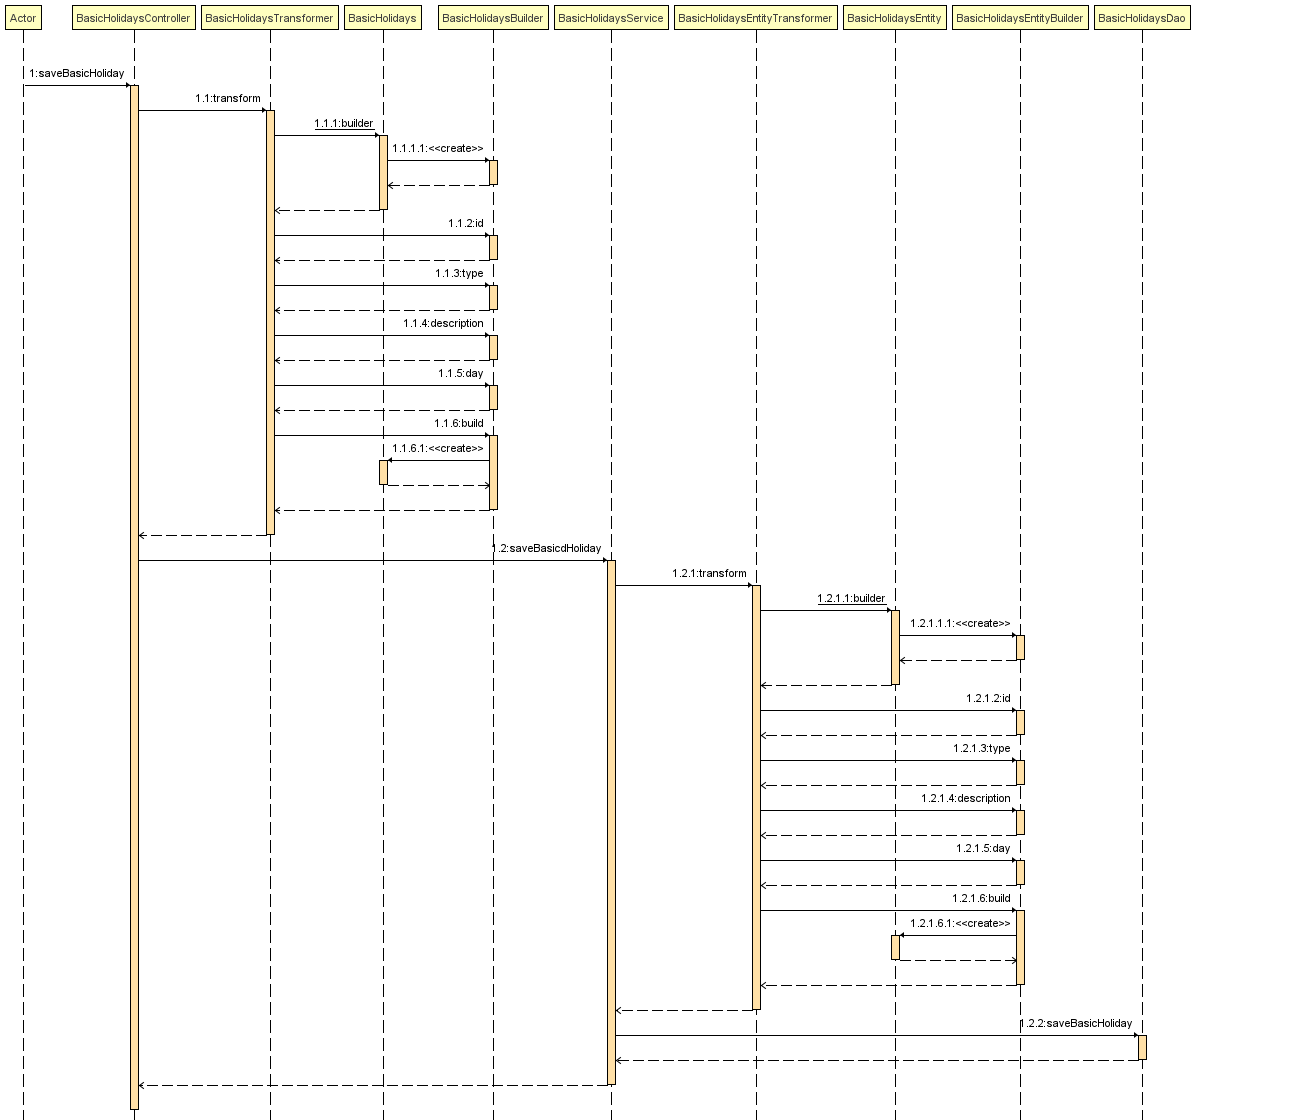
\includegraphics[scale=0.3]{images/teljesSzekvencia.png}
	\caption{HTTP Post kérés szekvenciája}
	\label{fig:teljesszekvencia}
\end{figure}

Lekérdező hívás esetén kihagyható a Belső objektumból Adatközvetítő objektumra való átalakítás, abban az esetben ha a belső objektum nem tartalmaz felesleges információt. Lényeges, hogy csak a szükséges adatokat továbbítsuk a megjelenítési réteg felé, felesleges adatok kiküldése szintén biztonsági problémát okozhat és sokkal jobban lassíthatja a megjelenítést mint a szerver oldali átalakítások. 

Az ehhez tartozó szekvenciadiagram látható \aref{fig:lekerdezoSzekvencia}. diagramon. 
\begin{figure}[h]
	\centering
	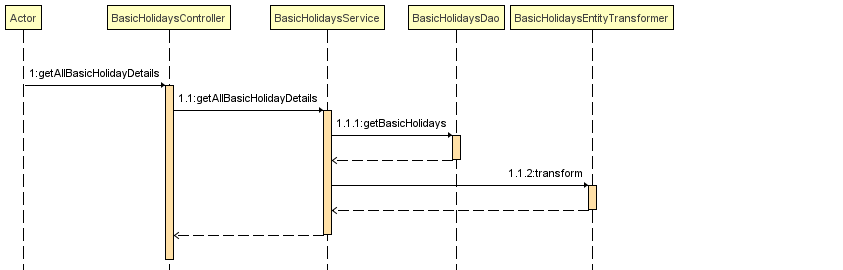
\includegraphics[scale=0.3]{images/lekérdezőSzekvencia.png}
	\caption{HTTP Get kérés szekvenciája}
	\label{fig:lekerdezoSzekvencia}
\end{figure}

Törlés esetén csak az adott elem azonosítóját várjuk paraméterként amit a gombnyomás automatikusan be tud küldeni, így validációra nincs szükség ezáltal a szekvencia is leegyszerűsödik. A törlés szekvenciája \aref{fig:törlesiSzekvencia}. diagramon látható.

\begin{figure}[h]
	\centering
	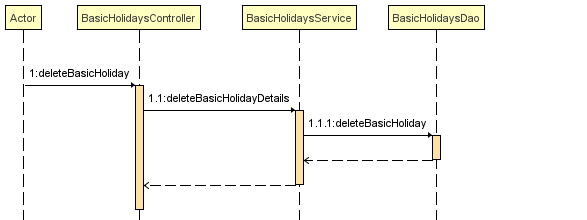
\includegraphics[scale=0.3]{images/törlésiSzekvencia.png}
	\caption{HTTP Delete kérés szekvenciája}
	\label{fig:törlesiSzekvencia}
\end{figure}

\Section{Adatbázis struktúra}
Webalkalmazások esetén az idő és erőforrás költség nagy részét az adatbázis műveleteken teszik ki, ezért fontos, hogy egyszerű és jól karbantartható struktúrát alakítsunk ki.
\vskip 0.2in
Az alkalmazáshoz tervezett adatbázis logikailag három részre bontható, kisebb önálló konfigurációs táblák,  felhasználókhoz tartozó adatok tárolása, valamint a jóváhagyási funkcióhoz szükséges táblák csoportja.

Minden logikai egység külön tervezési szemléletet igényel, ennek megfelelően az egységenkénti reláció megengedett, de az egységek közötti kapcsolatok kiépítése könnyen hibához vezethet.

\subsection{Konfigurációs táblák}

A korábban ismertetett szabadságolási szabályoknak megfelelően definiáltunk alap és pótszabadságot, valamint a pótszabadságon belül felsoroltunk több lehetőséget is, ezen lehetőségeknek saját értékeik és feltételeik vannak.

Alapvetően minden típushoz tartoznia kell egy egyedi azonosítónak és egy szám értéknek ami a szabadnapokat reprezentálja, ebből a tényből kiindulva érdemes lenne egy táblában tárolni az összes típust és megkülönböztetni azokat az egyedi értékeik alapján.

Ezzel a megoldással a következő problémák merülnek fel:
\begin{itemize}
	\item Az egyedi szabályozásokhoz saját értékek tartozhatnak, ebben az esetben komplex több oszlopos táblát kell létrehoznunk amiben kifejezetten sok null értéket tárolunk el.
	\item Minden lekérdezéskor összetett keresést kell alkalmaznunk, ha adott szabadságtípust keresünk.
	\item A tábla karbantartása komplikált feladat, ami redundanciához, és teljesítményromláshoz vezethet.
\end{itemize}

Ezáltal a tervezés során arra döntésre jutottam, hogy minden szabadság típus önálló adatbázistáblában definiálok, ahogy az \aref{fig:configurationUml}. diagramon látható. Ezáltal sok kisméretű táblát hozok létre, ezzel biztosítok jobb teljesítményt és költséghatékonyabb működést az applikációmnak ezen a területén. 

\begin{figure}[h]
	\centering
	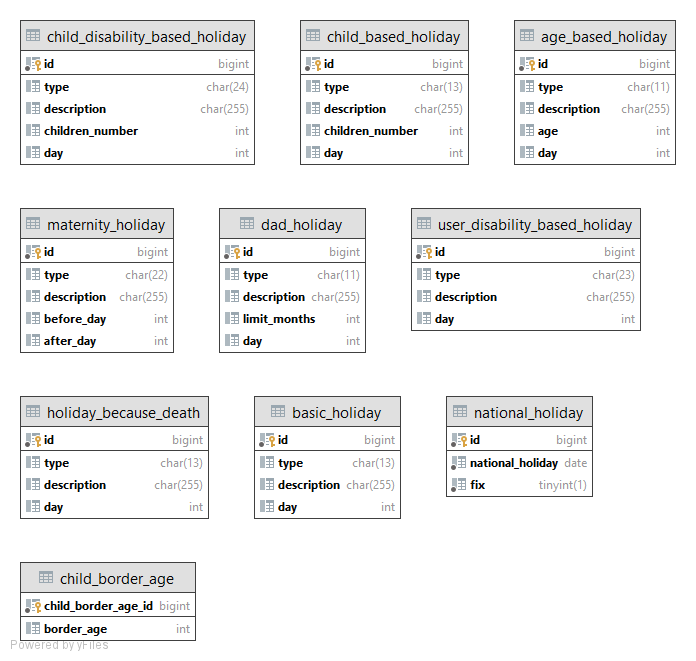
\includegraphics[scale=0.3]{images/configuration.png}
	\caption{Konfigurációs táblák UML diagramja}
	\label{fig:configurationUml}
\end{figure}

Továbbá a táblák tartalmát képezi egy típus érték is ami minden esetben konstansként jelenik meg és a pótszabadság típusát jelzi, ezzel az értékkel az automatizálási folyamat alatt megtudjuk különböztetni egymástól a típusokat.

Valamint minden tábla kapott egy leírás mezőt melyben a konfiguráció során elnevezhetjük az adott sort, hogy az egyes sorokat a felhasználó a felületen keresztül könnyebben megkülönböztesse.
\vskip 0.2in
Az időarányos szabadnapok számolásához, szükség van még a nemzeti ünnepek tárolása is, a tábla értéke megjelölhető egy boolean segítségével. \footnote{A boolean jelölés szerepét az implementáció alatt részletezem}

	Az alap szabadság esetén az adminisztrátor konfigurálhat egy 20 munkanapos szabadságot az "átlag" leírással, valamint egy 21 munkanapos sort is felvehet a "közalkalmazott" értékkel.


\subsection{Felhasználói adatok}

Az egység célja, hogy csak és kizárólag olyan adatot tároljunk a felhasználóról ami feltétlenül szükséges lesz az automatizáláshoz,mivel léteznek olyan pótszabadságok amik ha a jogszabály nem is változik maga a szabadság értéke függ a felhasználó bizonyos változó adataitól, ezért automatizálás szempontjából a változó adatokat állandó értékekből érdemes számolni a programban.

\begin{figure}[h]
	\centering
	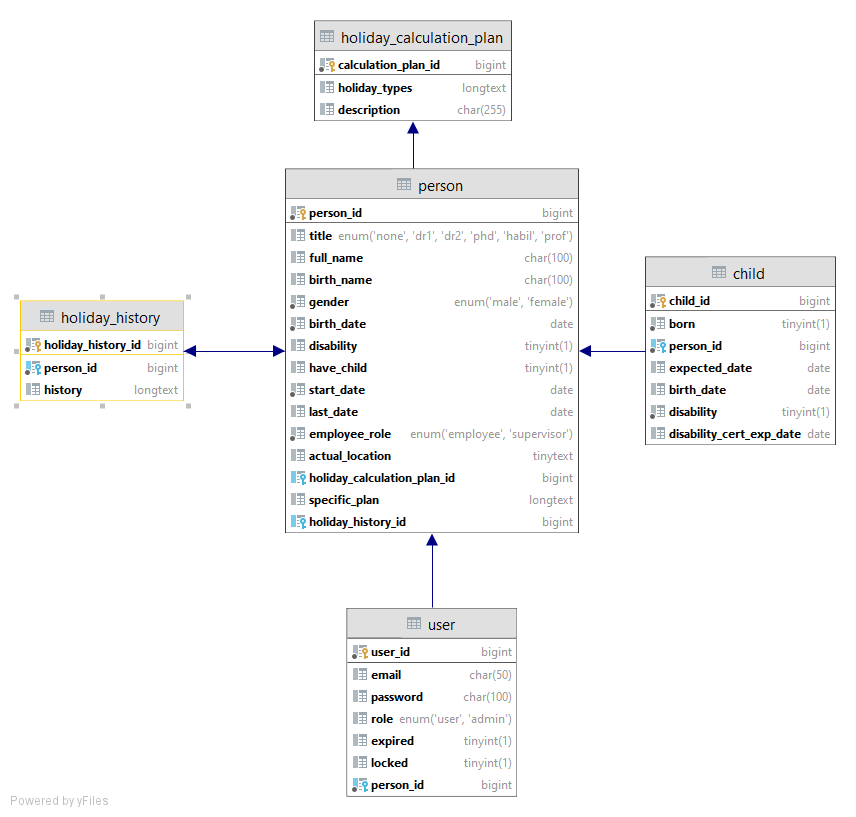
\includegraphics[scale=0.4]{images/felhasznalotablak.png}
	\caption{Felhasználóval kapcsolatos táblák UML diagramja}
	\label{fig:felhasznaloUML}
\end{figure}

A logikai egységet \aref{fig:felhasznaloUML} diagramon láthatjuk, a táblák egyéni szerepe:
\begin{itemize}
	\item \textbf{user:} A felhasználó beléptetése során az azonosítást szolgálja
	\item \textbf{person:} A felhasználó személyes adatai amik kalkulációkhoz és automatizáláshoz szükségesek.
	\item \textbf{child:} Ez a tábla egy több kapcsolatban áll a person táblával, mivel egy felhasználónak több gyermeke is lehet ennek függvényében eltérő pótszabadságokra jogosult
	\item \textbf{holiday\_calculation\_plan:} Ebben a táblában az adminisztrátor által meghatározott számítási formák vannak tárolva.\footnote{A fejezet későbbi részében részletesen kitérek rá.}, ez a tábla is egy több kapcsolatban áll a person-nel itt viszont, egy holiday\_calculation\_plan-hez tartozhat több felhasználó.
	\item \textbf{holiday\_history:} Mindenki egyéni szabadságolási története\footnote{A fejezet későbbi részében részletesen ismertetm}, éves felbontásban tárolja az egyénekre vonatkozó szabadságolási adatokat. 
\end{itemize} 
Érdemes még kitérni a "person" tábla néhány elemére:
\begin{itemize}
	\item \textbf{disability:} Pótszabadság illeti az alkalmazottat amennyiben valamilyen tartós egészségkárosodással él, mint például erőteljesen látás sérült.
	\item \textbf{have\_child:} A szülőis státusz gyors megállapítását hivatott biztosítani.
	\item \textbf{start\_date:} A munkaviszon kezdeti időpontja.
	\item \textbf{last\_date:} A munkaszerződés utolsó napja. (Opcionális érték)
	\item \textbf{employee\_role:} A felettes beosztott viszony definiálásában segít.
	\item \textbf{specific\_plan:} Az általános holiday\_calculation\_plan speciálisan a felhasználóra alakított változata.\footnote{A dolgozat későbbi részében részletesen bemutatom.}
\end{itemize}

Mindezek mellett, a "child" tábla is összetett adatokat tartalmaz:
\begin{itemize}
	\item \textbf{born:} Megmutatja, hogy a szóban forgó gyermek, megszületett-e már.
	\item \textbf{expected\_date:} A születés várható időpontja (Csak akkor létezik, ha born = false).
	\item \textbf{birth\_date:} A születési dátum, több felhasználási módja is van (Csak akkor létezik ha born = true).
	\item \textbf{disability:} Amennyiben a gyermek tartós fogyatékkal él a szülőt pótszabadság illeti.
	\item \textbf{diability\_cert\_exp\_date:} A szülő köteles bemutatni a gyermeke tartós hátrányos helyzetéről szóló határozatot, ennek egyes esetekben van lejárati ideje.
\end{itemize}
\subsection{Összetett adatok tárolása kisméretű táblákban}
Bizonyos objektumok túlságosan összetettek ahhoz, hogy ezeket egy a már bemutatott egyszerűsített adatbázisban tároljunk, amennyiben összetett egy több kapcsolattal teletűzdelt adatbázisrendszerben valósítjuk meg, az könnyedé vezethet rendkívül bonyolult struktúrát, és hosszan tartó komplex lekérdezéseket.

Megfigyelhető \aref{fig:felhasznaloUML} diagramon, hogy a \textbf{holiday\_types}, \textbf{specific\_plan}, és a \textbf{history} mezők longtext érték definíciót kaptak. Ez a tervezési döntés azért született, hogy az applikáció Belső objektumaiban bonyolult osztályhierarchiában álló adatokat egyetlen JSON-ben tudjam tárolni.

Ezzel a megoldással több tábla és több-száz sornyi adatbázis rekord létrehozását és tárolását kerülöm el, nem csak a nagy mennyiségű tárhelyet csökkentem hanem a lekérdezések bonyolultságát is, ezzel együtt az applikáció teljesítménye is növekszik.

Fontos megemlíteni, hogy ez a tervezési döntés nagyban hozzájárul az automatizálás megvalósításához, mivel az időigényes adatbázis műveletek lecsökkennek egyetlen lekérdezésre, aminek a végén a String típusú eredményből könnyen kezelhető objektum keletkezik.

\subsection{Jóváhagyáshoz szükséges táblák}
Ma a szoftverfejlesztésben gyakori igényt képez, hogy a felettesek jóváhagyják beosztottaik különböző kéréseit, ez önmagában komoly tervezést igénylő probléma, viszont megoldható egy létező ingyenes API hívással ami a saját adatbázisunkban dolgozik. A kiszolgáló legenerálja a számára szükséges táblákat és menedzseli azokat.\cite{flowable}

\Section{Funkció tervezés}

Az elvégzett igényfelmérés, és a már létező megvalósítások alapján részletesen specifikálhatóak azok a funkciók amelyek teljes megvalósítása esetén az applikáció teljesen elkészültnek minősíthető. Lényeges megemlíteni, hogy amennyiben a megvalósítás során megfelelő fontossági sorrendet tudunk állítani elérhető az a pont a fejlesztésben, ahonnan a program üzembe helyezhető. Ezzel már nagyban könnyíteni a felhasználók munkáját, amíg a további fejlesztések folynak.

Minden itt leírt funkció esetén megvalósításnál a fejezet elején lefektetett architektúra követése az elvárt működés része.

\subsection{Felhasználó és hozzáférés kezelés}

A szoftverbiztonság kiemelten fontos még a belső hálózaton működő rendszereknél is, viszont amennyiben a Webapplikációnk nyilvános címen üzemel a hozzáférés kezelés elengedhetetlen. 

A program ezzel kapcsolatos működési követelményei:
\begin{enumerate}
	\item A felhasználó egyedi felhasználónév és jelszó segítségével be tud jelentkezni a felületre, továbbá van kijelentkezési lehetősége is.
	\item Minden felhasználó csak és kizárólag a jogkörének megfelelő oldalakhoz és funkciókhoz fér hozzá.
\end{enumerate}

\paragraph{Adminisztrátor jogkör}
Többnyire az intézeti/tanszéki adminisztrátor tölti be ezt a szerepet, ehhez a jogkörhöz tartozik, a legtöbb hozzáférés és funkció.
\subparagraph{Felhasználó létrehozása}
Alapvető adminisztrátori feladat, amely során a külön erre létrehozott menüpont alatt az ügyintéző megadja a következő felhasználói adatokat:
\begin{itemize}
	\item egyedi email címe,
	\item teljes neve,
	\item jogköre.
\end{itemize}
A létrehozás gombra kattintva, a program létrehozza az adatbázisban az új felhasználót.

\subparagraph{Felhasználó adatainak lekérdezése és módosítása}
Az adminisztrátor megnyithatja az a menüpontot ahol kilistázzuk az összes alkalmazottat, a listában tud keresni, megfelelő gombra kattintva tovább navigáljuk a felhasználó részletese adatait tartalmazó oldalra, ahol a következő funkciókat tudja használni: 
\begin{itemize}
	\item felhasználói adatok szerkesztése és mentése,
	\item felhasználó gyermekeire vonatkozó adatok szerkesztése és mentése,
	\item adatok törlése,
	\item felhasználóhoz kapcsolódó szabadságra vonatkozó adatok hozzárendelése, generálása (specializált szabadság szabályzat). 
\end{itemize}

\subparagraph{Felhasználóra vonatkozó szabadságolási szabályok létrehozása}
Az adminisztrátor rendelkezik olyan funkcióval ahol menedzselhet szabadságolási szabályokat, amely tartalmazza a kiválasztott alap szabadságot, és a felhasználókra vonatkozó pótszabadságok típusainak listáját.

\paragraph{Felhasználó, felettes jogkör}
Ebben a jogkörbe tartozik a szervezeti egység vezetője, lekérdezheti az beosztottak listáját, és azok szabadság történetét.

\subparagraph{Alkalmazotti kérések bírálása}
A felettes rendelkezik olyan menüponttal, ahol lista nézetben láthatja a beosztottak szabadságolással kapcsolatos kérelmeit, azokon a következő műveleteket tudja végezni:
\begin{itemize}
	\item Kérelem elfogadása,
	\item Kérelem visszautasítása,
	\item Visszautasítás indoklása.
\end{itemize}

\subparagraph{Éves szabadságterv készítése és módosítása}
Elérhető egy felület ahol naptár nézetben jól elkülöníthető színekkel jelezve könnyen szerkeszthető és menthető az éves szabadságolási terv.

\paragraph{Felhasználó, beosztott jogkör}
A legtöbb felhasználó ebbe a jogkörbe tartozik, az általuk látható és használható funkciók a legkevesebb.

\subparagraph{Saját adatok lekérdezése}
A felhasználó bármikor lekérdezheti, de nem módosíthatja az adatokat amiket az adatbázisban tárolunk róla.

\subparagraph{Saját szabadnapok kiírása, nyomon követése}
A korábban definiált szabályoknak megfelelően képes létrehozni szabadnapokat, amelyek a felettesi bíráláson keresztül mennek, a már létrehozott szabadnapok módosítása újbóli bírálásra kerül. 

A felületen megtekintheti az éves szabadnapjainak a számát valamint a még fel nem használt napok is kijelzésre kerülnek.
\vskip 0.2in
Fontos, hogy ezek a funkciók a többi jogkörben is elérhetőek! 

\subsection{Szabadságolási szabályok konfigurálása}
Kulcsfontosságú funkció ami az adminisztrátori jogkör alá tartozik.

\paragraph{Alap és pótszabadságok}
Minden szabadságtípushoz tartozik egy egyedi, különálló felület ahol a szabályoknak megfelelően szerkeszthetőek, minden esetleges további konfiguráció jól érthető külön felületen van létrehozva.

	Alapszabadság konfigurálásához a felhasználó a következő lépéseket kell végrehajtsa:
	\begin{enumerate}
		\item Elnavigál az alapszabadságok menüpont alatt a listanézetre
		\item A hozzáadás gombra kattintva átirányítjuk az alapszabadság létrehozása űrlaphoz.
		\item A felület kitöltése után rákattint a mentés gombara.
		\item Sikeres végrehajtás esetén átirányítjuk a listanézetre, ellenkező esetben a megfelelő hibaüzenettel tájékoztatjuk.
	\end{enumerate}

\paragraph{Nemzeti ünnepek}
Ezen dátumok ismerete fontos részét képezik az éves szabadság arányos számolásának, rendkívül fontos az automatizálás szempontjából, hogy minden évben a valóságot tükrözze az általunk tárolt adat.

Az elvárt működésnek több megvalósítási lehetősége van:\footnote{A megvalósítás alatt ezekkel a lehetőségekkel részletesen foglalkozok.}
\begin{enumerate}
	\item Az adminisztrátor kézzel konfigurálja ezeket az adatokat minden évben.
	\item A manuális konfiguráció során megjelöljük a nem mozgó dátumokat amit automatikusan újra tudunk számolni, minden mást évente kézzel konfigurál a felhasználó.
	\item Az állandó dátumokat SQL segítségével beégetjük az adatbázisba, a mozgó dátumokat újraszámoljuk.
	\item Külső API hívás segítségével lekérdezzük minden év elején az adatokat amikre kíváncsiak vagyunk. 
\end{enumerate}

\subsection{Automatizált működés}
A rendelkezésre álló információk alapján az automatizálható funkciók főként az éves kalkulációkkal és tervezési munkálatokkal kapcsolatosak, ezeken felül viszont mindennapos automatizált futással a gyermekszületéssel kapcsolatos adatok alapján automatizálható az ehhez kacsolódó esemény alapú pótszabadságok kezelése is.

\paragraph{Éves szabadnapok időarányos számolása}
Ez a funkció csak részben automatizálható, amennyiben az adminisztrátor év közben hoz létre felhasználót abban az esetben biztosítanunk kell egy gombot számára amivel lehetősége nyílik az azonnali számolások elindítására.

Az automatizálással kapcsolatos műveletek a következők:
\begin{enumerate}
	\item Minden év utolsó napjának a végén a megfelelő számolást és módosítást végző funkciók futása,
	\item A felhasználóhoz rendelt szabályok, specializált formájának aktualizálása.
	\item Az aktualizált szabályok alapján az éves szabadság kiszámolása.
	\item Az éves szabadság arányos újra számolása tört év esetén.
	\item Az új éves történet létrehozása, és az éves szabadságkeret hozzáadása.
	\item Szabadság történet frissítése és mentése a megfelelő felhasználóhoz csatolva.
\end{enumerate}

\paragraph{Születéssel kapcsolatos szabadnapok esemény alapú kezelése}
Ez az automatizálás napi szintű futtatást igényel ezeket az ellenőrzéseket nap végén érdemes elvégezni.

A tervezett működés lépései a következőek\footnote{Férfiak és nők esetén a szabályozások különböznek így a megvalósításban pontosabb képet kaphatunk a témáról.}:
\begin{enumerate}
	\item Az érintett alkalmazottak kikeresése.
	\item A szabályozásnak megfelelő szabadságok létrehozása
	\item Az éves történet módosítása, és mentése.
	\item Esetleges utólagos ellenőrzések elvégzése.
\end{enumerate}

\paragraph{Éves szabadságterv generálása}
Ennek a funkciónak az automatizálása, a legösszetettebb, mivel nem csak az országos szabályozásoknak de az intézmény szabályainak is eleget kell tennünk.

Az automatizált futásnak minden év december 31. előtt meg kell történnie, a tervezett lépései:
\begin{enumerate}
	\item Az összes felhasználó lekérdezése.
	\item A felhasználók adatainak frissítése.
	\item Éves szabadság egyenlegük arányos kiszámolása.
	\item A szabadnapjaik beosztása a 7-14 napos szabálynak megfelelően.
	\item Az egyetemi szabályzatban előírtak betartása.
	\item Szabadságterv mentése egy saját adatbázis táblába.
\end{enumerate}
\subsection{Szabadságolási statisztikák készítése}
Az adminisztrátor jogkörrel rendelkező felhasználónak elérhető, egy menüpont az oldalon, ahol statisztikákat tud generálni az intézet alkalmazottainak adatai alapján.

A funkcióban a következő működések szerepelhetnek:
\begin{itemize}
	\item Statisztika kimenetének kiválasztása(diagramok, táblázatok, esetleg formanyomtatványok),
	\item Adatok intervallumának dinamikus állíthatósága,
	\item A statisztikák alanyainak beállítása.
\end{itemize}

\Chapter{Az alkalmazás megvalósítása Java Enterprise környezetben}

\Section{Mappastruktúra kialakítása}
A jól strukturáltság fontos szempont az implementáció alatt, mivel az osztályok konzisztens elnevezésével funkciónak megfelelő elhelyezésével a fejlesztési folyamat során könnyebben azonosíthatjuk az elhelyezkedésüket.

\subsection{Modularizált alkalmazás}
Az alkalmazásunk viselkedés alapján való modulokra bontása jól elkülöníthetővé teszi a különböző szerepkörű implementációkat, és a maven segítségével biztosíthatjuk, hogy a modulok lássák egymást.
 
\begin{figure}[h]
	\centering
	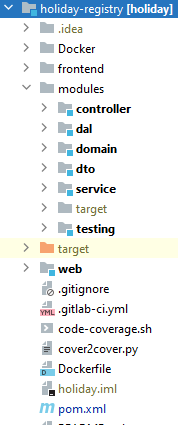
\includegraphics[scale=0.6]{images/mapstructure.png}
	\caption{Modularizált alkalmazás mappastruktúrája}
	\label{fig:mapstructure}
\end{figure}

A már részletesen ismertetett Többszintű alkalmazás felépítését tükrözi \aref{fig:mapstructure}. ábra. 
Az itt látható felosztásban a gyökér könyvtáron belül található a web module aminek jelenesetünkben csak konfigurációs szerepe van, mivel a spring-boot alkalmazások esetén a main függvényt tartalmazó osztálynak a csomaghierarchia legkülső csomagjában kell elhelyezkednie.

Amennyiben ez nem megfelelő helyen található az alkalmazásunk nem fogja látni a létrehozni kívánt komponenseket és a kontextust nem tudja felépíteni.

\paragraph{Frontend mappa}
Szintén leolvasható \aref{fig:mapstructure}. ábráról, hogy a jelen esetben struktúra részét képezi a megjelenítési réteghez szükséges applikációt tartalmazó mappa is. Mivel jelenleg nem microservice architektúrát alkalmazunk ez a megoldás is elfogadható, de gyakorlatban nem ajánlott és igen ritka.

\paragraph{Testing}
Ez egy úgynevezett rétegeken átívelő modul, aminek minden rétegben szerepe van, ebben a megvalósításban a modul nem tartalmaz kódot, csupán konfigurációt és a maven jacoco nevezetű teszt riport generáló kiegészítője által létrehozott fájlokat. Ezeket a fejlesztés során a tesztlefedettség méréséhez használjuk, képes vizualizációi segítségével megmutatni egy html oldalon, melyik osztályban milyen szintű a lefedettség, és azt is milyen hiányosságaink vannak tesztek terén.

\Section{Összetett objektum előállítása JSON formátumból Lombok használatával}

A szoftverfejlesztés egyik alapelve az, hogy ne ismételd önmagad, ami a redundanciából eredő hibalehetőségek és fejlesztési komplikációk csökkentése érdekében lett egy kitűzött cél. Az elv ellenére mégis rengeteg egyszerű kódsort ismételünk újra az Objektum Orientált fejlesztés során.

\subsection{Az ismétlődő programrészletek}

Minden általános java objektum létrehozásakor létrehozunk az osztály mezőihez:
\begin{itemize}
	\item legalább egy konstruktort,
	\item beállító és lekérdező függvényeket,
	\item titkosító valamint egyenlőség vizsgáló függvényeket,
	\item és a könnyebb hibakeresés érdekében, még egy kiíró függvényt is.
\end{itemize}

Ezek az implementációk legtöbbször annyira elemiek, hogy minden fejlesztőkörnyezet, automatikusan képes generálni a hozzájuk tartozó implementációt. Ez a sokszor több száz sornyi kódrészlet rengeteg tárhelyet jelent valamint tesztelés szempontjából ezek az osztályok többnyire rontják a lefedettséget. Mivel ezeknek a függvényeknek a tesztelése a nyelv működésére irányulna, így a saját alkalmazásunkban felesleges ezekre tesztesetet implementálni.

\subsection{A Lombok működése}
A felvázolt probléma megoldására született a Project Lombok\cite{lombok} könyvtár aminek a segítségével egyszerű annotációk használatával használhatjuk ezeket a kódrészleteket anélkül, hogy implementálnánk azokat a saját programunkban

\paragraph{@Data} használatával a mezők definiálása után rögtön használhatóvá válnak a már említett redundánsnak mondható kódok.
\begin{java}
	@Data
	public class UserEntity {
		private Long userId;
		private String email;
		private String password;
		private UserEntityRole role;
	}
	
\end{java}

\subsection{Megváltoztathatatlan objektumok Lombokban}
Objektum orientált programozásban gyakran használunk objektumokat adatok továbbítására, adattovábbítás esetén fontos, hogy gondosodjuk az objektum állapotáról. Amennyiben az változtatható a programozás, abban az esetben megnövekszik a hibalehetőségek száma.
\vskip 0.2in
Ahhoz, hogy ne lehessen bármikor megváltoztatni egy objektum mezőjének az állapotát, úgy kell megírni a hozzá tartozó függvényeket, hogy a mezőértékek csak és kizárólag a referencia létrehozásakor legyenek beállíthatóak.

A megoldás egy része igen egyszerű nem, hozunk létre olyan függvényeket ami példányosítást követően módosítani tudja az állapotot, tehát a beállító vagy más néven set függvényeket nem implementáljuk.

Ezáltal, viszont konstruktor argumentumokon keresztül lehet csak példányosítani, és ha esetleg adott esetben az egyik paraméter nem létezik ott, a példányosításkor null értéket kell átadnunk. Továbbá a paraméter sorrend is gondot okozhat ezért ez egy körülményes megoldás.

\paragraph{Építő minta} segítségével pontosan láthatjuk melyik mezőt definiáljuk és melyiket nem, ebben a megoldásban egy privát konstruktoron keresztül példányosítjuk az osztályunkat aminek a belső builder azaz epítő osztályán keresztül állítunk be.

\vskip 0.2in
Ez ismét a korábban említett problémakörhöz vezet, ezért a Lombok könyvtár erre is nyújt megoldást a \textbf{@Value} valamint a \textbf{@Builder} elölések használatával. 

Amíg az előbbi a megváltoztathatatlan osztály feltételeit teremti meg addig az utóbbi segítségével egy könnyen használható építő mintát megvalósító belső osztályt kapunk.

\subsection{JSON felépítésű String generálása Jacksonnal}

A Jackson könyvtár egy olyan megvalósítást kínál ami segítségével könnyedén alakíthatjuk át összetett java objektumainkat egy egyszerű JSON formátumú String értékké. 

Ennek a könyvtárnak a segítségével Belső modulban létező Holidayhistory.java osztályban található összetett objektum könnyedén átalakítható egy egyszerű String típussá és bármikor elvégezhető az átalakítás visszafelé is. 

A következő osztály struktúrából:
\begin{java}
public class HolidayHistory {	
	Long id;
	PersonDetails person;
	List<YearHistory> yearHistories;
}

public class YearHistory {
	int year;
	BigDecimal fixHolidaysForTheYear;
	List<EventRelatedHoliday> eventRelatedHolidays;
	List<HolidayEvent> holidayEvents;
}

public class EventRelatedHoliday {
	EventRelatedHolidayType holidayType;
	int days;
	LocalDate eventDate;
	LocalDate expiration;
}

public class HolidayEvent {
	String description;
	LocalDate startDate;
	LocalDate endDate;
	Boolean dadHoliday;
}
\end{java}

Az itt látható JSON értéket generálja ami már könnyedén menthető az adatbázisunkban.
\begin{java}
[
{
	"year": 2020,
	"fixHolidaysForTheYear": 10,
	"eventRelatedHolidays": [
	{
		"holidayType": "dad",
		"days": 0,
		"eventDate": "2021-03-30",
		"expiration": null
	},
	{
		"holidayType": "dad",
		"days": 0,
		"eventDate": "2021-03-30",
		"expiration": "2021-04-10"
	}
	],
	"holidayEvent": [
	{
		"description": "desc",
		"startDate": "2020-03-04",
		"endDate": "2020-05-20",
		"dadHoliday": null
	}
	]
},
{
	"year": 2021,
	"fixHolidaysForTheYear": 10,
	"eventRelatedHolidays": [
	{
		"holidayType": "dad",
		"days": 0,
		"eventDate": "2021-03-30",
		"expiration": null
	},
	{
		"holidayType": "dad",
		"days": 0,
		"eventDate": "2021-03-30",
		"expiration": "2021-04-10"
	}
	],
	"holidayEvent": null
}
]
\end{java}

A Jackson elap beállítás esetén a JSON létrehozásához a lekérdező függvényeket használja, így egyértelmű, hogy a JSON formátumból a beállító függvények segítségével állít elő objektumot.

Ahhoz, hogy a lombok és Jackson könyvtárak megfelelően működjenek együtt Megváltoztathatatlan objektumok létrehozása esetén az építő függvény további beállításaira valamint új annotációk használatára van szükségünk.

Minden érintett osztályt a következő alakra kell hozni.
\begin{java}
@Value
@Builder(builderClassName = "YearHistoryBuilder", 
access = AccessLevel.PUBLIC)
@JsonDeserialize(builder = 
YearHistory.YearHistoryBuilder.class)
@AllArgsConstructor(access = AccessLevel.PRIVATE)
public class YearHistory {
	
	@JsonProperty("year")
	int year;
	@JsonProperty("fixHolidaysForTheYear")
	BigDecimal fixHolidaysForTheYear;
	@JsonProperty("eventRelatedHolidays")
	List<EventRelatedHoliday> eventRelatedHolidays;
	@JsonProperty("holidayEvent")
	List<HolidayEvent> holidayEvents;
	
	@JsonPOJOBuilder(withPrefix = "")
	public static class YearHistoryBuilder {}
}
\end{java}  

Az itt látható alakban a Jackson könyvtár már képes azonosítani az átalakításhoz szükséges Lombok által biztosított függvényeket.

\Section{Automatizált Cron munkamenetek Springben}

Az automatizálás kulcsfontosságú szerepet játszik az alkalmazás piaci rést betöltő lehetőségeiben, ezért kifejezetten fontos, hogy a beállított időzített processzek fond nélkül végrehajtódjanak.

\paragraph{Java timer} segítségével képesek vagyunk másodpercben definiálni egy időzítőt ami az első indítástól számítva minden alkalommal folyamatosan számol és az időzítő lejártakor elindíthatunk egy feladatot vagy komplex feladat sort is.

Sajnos ez a megoldás nem megfelelő számunkra hiszen az időzítő minden újrainduláskor lefutna valamint akár kiszámíthatatlan viselkedést is generálhat.

\subsection{A keretrendszer nyújtotta előnyök}
A Spring keretrendszerben sok megbízható és könnyen alkalmazható megoldás található már létező problémákra, ezek közé tartozik az automatizált függvényhívások is.
\vskip 0.2in
A megoldás során a keretrendszer egy Cron munkamenetet, hoz létre az általunk konfigurált futási feltételeknek megfelelően, ez esetben nem az applikáció belső számlálója felel a függvényhívás elindításáért. A munkamenet a szerver számítógépen jön létre és minden alkalommal meghívja azt a függvényt amelyiken definiáltuk amennyiben az aktuális dátum és idő egyezik az általunk konfigurálttal.

\subsection{Cron munkamenet implementálása Spring-boot-ban}

A spring-boot applikáció indító függősége automatikusan tartalmazza a számunkra szükséges könyvtárakat, viszont az eléréséhez és használatához meg kell jelölnünk a megfelelő osztályokat és függvényeket.

\begin{java}
	@SpringBootApplication
	@EnableScheduling
	public class HolidayApplication {...}
\end{java}

Engedélyezést követően az applikáció kontextusában bármelyik nyilvános függvényünk megjelölésével létrehozhatunk egy új munkamenetet.

\begin{java}
@Scheduled(cron = "1 0 0 * * ?")
public void schedule() {
	unusedHolidaysService.addPenalty();
	childBornHolidaysService.validate();
}
\end{java}

Léteznek előre definiált beállítások z automatizált futtatáshoz, de ahogy a kódrészlet is mutatja bármikor konfigurálhatunk saját feltételeket, a cron leírónyelv segítségével.

A nyelvben hat karaktert kell megadnunk amik jelentését \aref{tab:Cron leírónyelv} táblázat tartalmazza:

\begin{table}[h]
	\centering
	\caption{Cron leírónyelv értékei.}
	\label{tab:Cron leírónyelv}
\begin{tabular}{|c|c|c|c|}
	\hline
	Érték & Kötelező & Megengedett értékek & Speciális karakterek \\
	\hline
	Másodperc & Igen & 0-59 & , - * / \\
	\hline
	Perc & Igen & 0-59 & , - * / \\
	\hline
	Óra & Igen & 0-23 & , - * / \\
	\hline
	Hónap napja & Igen & 1-31 & , - * ? / L W C \\
	\hline
	Hónap & Igen & 0-11 vagy JAN-DEC & , - * / \\
	\hline
	Hét napja & Igen & 1-7 vagy SUN-SAT & , - * ? / L C \# \\
	\hline
	Év & Nem & üres vagy 1970-2099 & , - * / \\
	\hline
\end{tabular}
\end{table}

\Section{Automatizált szabadság számolás tört év esetén, Nemzeti ünnepek tárolása}

Az automatizálás folyamatát és a törvényben leírt szabályoknak megfelelő számítást ismerve könnyedén megvalósíthatunk egy összetett hívási láncot amely végén az éves vagy akaár a részarányos szabadnapok számolása megtörténik.
A kihívást jelentő probléma az egyenletben egyedül, az aktuális éveben hátralévő munkanapok száma jelenti, ehhez ugyanis minden számolás esetén tudnunk kell a tárgy évben mennyi olyan munkanap létezik amely az aktuális nemzet számára munkaszüneti napnak minősül.
\vskip 0.2in
Habár a szóban forgó dátumok többsége állandó és az ezekre vonatkozó megoldás kézenfekvő, mozgó ünnepek esetén nem tárolhatunk állandó értéket. 

\subsection{Külső API hívása}
Kisebb kereséssel rengeteg számunkra hasznos szolgáltatást találhatunk ahol, egy bizonyos URL összeállításával és a mögötte található végpont meghívásával minden szükséges információhoz hozzájuthatunk.

A legegyszerűbb verzió visszatérési értéke teljes mértékben tökéletes lenne számunkra hiszen tartalmazza azt a számot amit felhasználva csak be kell helyettesítenünk az egyenletünkbe.

Több lehetőség van amelynél az adott év vagy nap adatainak megadása esetén visszakapjuk, hogy az munkanap vagy sem.
\vskip0.2in
A legnagyobb probléma viszont ezekkel az elérhető alkalmazásokkal, hogy az ingyenes hozzáférésük szigorúan korlátozva van, havi vagy éves előfizetésük pedig jelen esetben nem összeegyeztethető ár érték arányban az igényeinkkel.

\subsection{Mozgó ünnepek számolása}

A külső API hívások nélkül a legkézenfekvőbb megoldása az automatizálásnak, hogy saját magunk számoljuk ki az adott dátumok értékeit, ehhez könnyedén találhatunk számolásokat. 

Ezekről a számolásokról viszont elmondhatjuk, hogy nem adnak valós értéket, különböző tényezők miatt hónapokat tévedhetnek, így kis utánajárással kideríthetjük, hogy a jelenleg kiszámolt mozgó ünnepek dátumai egyrészt számoláson másrészt megegyezésen alapulnak.

Kimondhatjuk tehát, hogy saját számolások elvégzése, jelen esetben nem megvalósítható.

\subsection{Félautomata megoldás}

A végleges megoldás egy részben manuális karbantartást igénylő implementáció, melynek során az állandó dátummal rendelkező dátumok első beállítást követően újra számolódnak, a nem változó dátum jelölés esetén viszont az adminisztrátorra bízzuk a konfigurációt.

\Section{Folyamatos Integráció beállítása Gitlabon}

A már említett CI/CD folyamatok beállítása nagy segítséget tud nyújtani és a fejlesztést is meggyorsíthatja, a kódbázis felépítése és a tesztek futtatása idő és erőforrás igényes lehet a saját számítógépünkön, így ezt a munkát delegálva időt nyerhetünk. 

A gitlab verziókezelő szolgáltatás lehetőséget nyújt saját Folyamatos integrációs csővezeték definiálásra amiben, az építés, a tesztek futtatása és a generált adatok alapján a tesztlefedettséget mérő munkameneteket könnyedén definiálhatjuk.

\subsection{.gitlab-ci.yml konfiguráció}

A gitlab szolgáltatásának részét képezi az alap szintű integrációs folyamatok létrehozása, ezek indulása automatikus. Nekünk csupán egy konfigurációs .yml kiterjesztésű fileban kell definiálnunk az általunk futtatni kívánt folyamatokat és az azokhoz tartozó esetleges környezeti változókat, vagy parancsokat.

A stages érték megadása után definiálnunk kell a munkamenetek nevét és sorrendjét.
 \begin{python}
 	stages:
 	  - build
 	  - test
 	  - coverage
 \end{python} 

Ezután konfiguráljuk a munkamenet, úgy hogy hivatkozunk a nevére majd megadjuk, hogy milyen docker image környezetben fusson az adott folyamat.

\begin{python}
	build:
	  stage: build
	  image: maven:3.6.3-jdk-11
\end{python}

Legvégül a script érték alatt  felsoroljuk milyen parancsokat hajtson végre a docker imagen belül. 
\begin{python}
	script:
	  - mvn $MAVEN_CLI_OPTS compile
	  
\end{python}

\subsection{További felhasználható funkció}
Ez a gyors konfiguráció nem csak a fejlesztést gyorsíthatja fel de akár Folyamatos szállítást is definiálhatunk vele, egy olyan munkamenet segítségével ami a felépített alkalmazásunk futtatható .war vagy .jar kiterjesztésű futtatható elemeit becsomagolja egy docker konténerbe, ssh kapcsolatot létesít egy általunk definiált IP címmel és ott a megadott helyre kitelepíti az alkalmazásunkat.

Ezzel elérhetjük, hogy a felhasználó a nap végére akár több hibajavítás eredményét vagy akár pár hetente egy új funkció használatát is élvezhesse. 
\Chapter{Rest applikáció tesztelése}

\Section{Unit tesztek}

A fejlesztés során folyamatos logikai egység tesztek írása már fejlesztési időben jelentős mennyiségű tervezési és megvalósítással kapcsolatos hibára mutat rá.

A megvalósítás részeként a konfigurációs és kizárólag nyelvi elemeket tartalmazó osztályok kivételével, folyamatos tesztlefedettség ellenőrzéssel történt az implementáció.

\vskip 0.2in
A kódbázis, összesen 312 db egység tesztet tartalmaz, amelyek a mérések alapján 99\%-os tesztlefedettséget jelentenek.
Mint ahogy azt \aref{fig:jacocoReport} ábra is mutatja.

\begin{figure}[h]
\centering
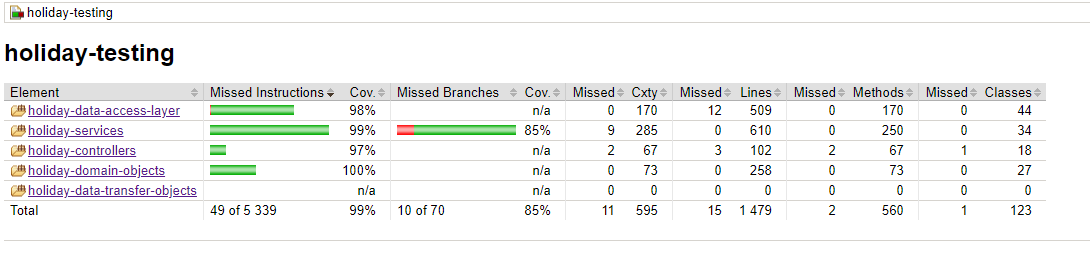
\includegraphics[scale=0.5]{images/jacocoReport.png}
\caption{Jacoco riport generált adatai.}
\label{fig:jacocoReport}
\end{figure}

Az alkalmazás teljes felépítése a tesztek futtatásával átlagosan 40 és 45 másodperc közé tehető.

\Section{Funkcionális tesztek Swagger UI segítségével}

A WEB applikációk szerver oldali logikája megjelenítési rétegtől függetlenül tesztelhetőek, az általunk létrehozott végpontok erre alkalmas programok segítségével és a megfelelő HTTP kérésekkel meghívhatóak és a program futási időben kiszolgálja azokat.
\vskip 0.2in

Ahhoz, hogy ne kelljen külső programot használni egy külső könyvtár segítségével saját felületet generálhatunk az végpontjaink számára. A kontextus épülésekor a külső függőség meghívódik és az általunk vezérlő típusként definiált osztályok HTTP hívással megjelölt függvényei alapján megjelenítést generál ami jól látható \aref{fig:swaggerUI}. 

\begin{figure}[h]
	\centering
	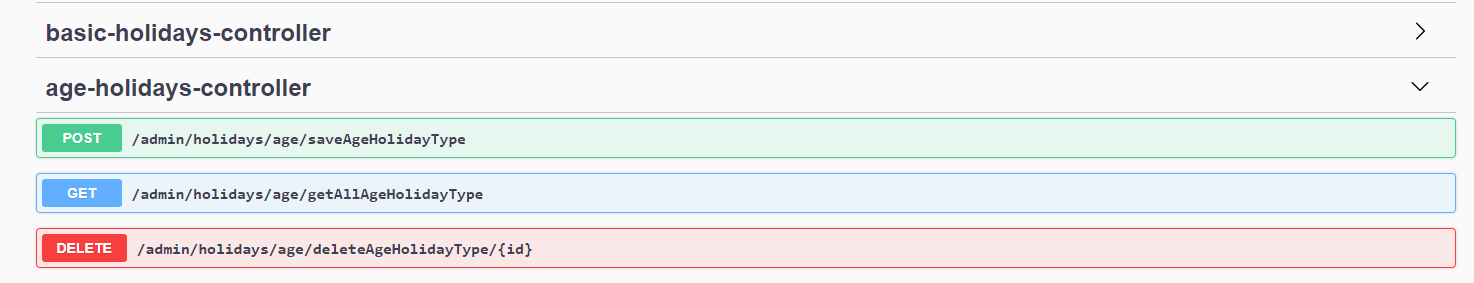
\includegraphics[scale=0.3]{images/swaggerUI.png}
	\caption{Swagger UI felület.}
	\label{fig:swaggerUI}
\end{figure}

Előnye, hogy nem csak láthatóvá teszi végpontokat, de dokumentációként is szolgál számunkra a bemeneti és visszatérési értékekről egyaránt. Továbbá biztosít még egy kitölthető űrlapot és egy mintát a aminek a segítségével a megfelelő JSON hívással ki is próbálhatjuk az adott funkció működését. 

A küldés \aref{fig:swaggerPostTest} ábrán \aref{fig:swaggerGetTest} pedig a lekérdezés tesztekése látható.

\begin{figure}[h]
	\centering
	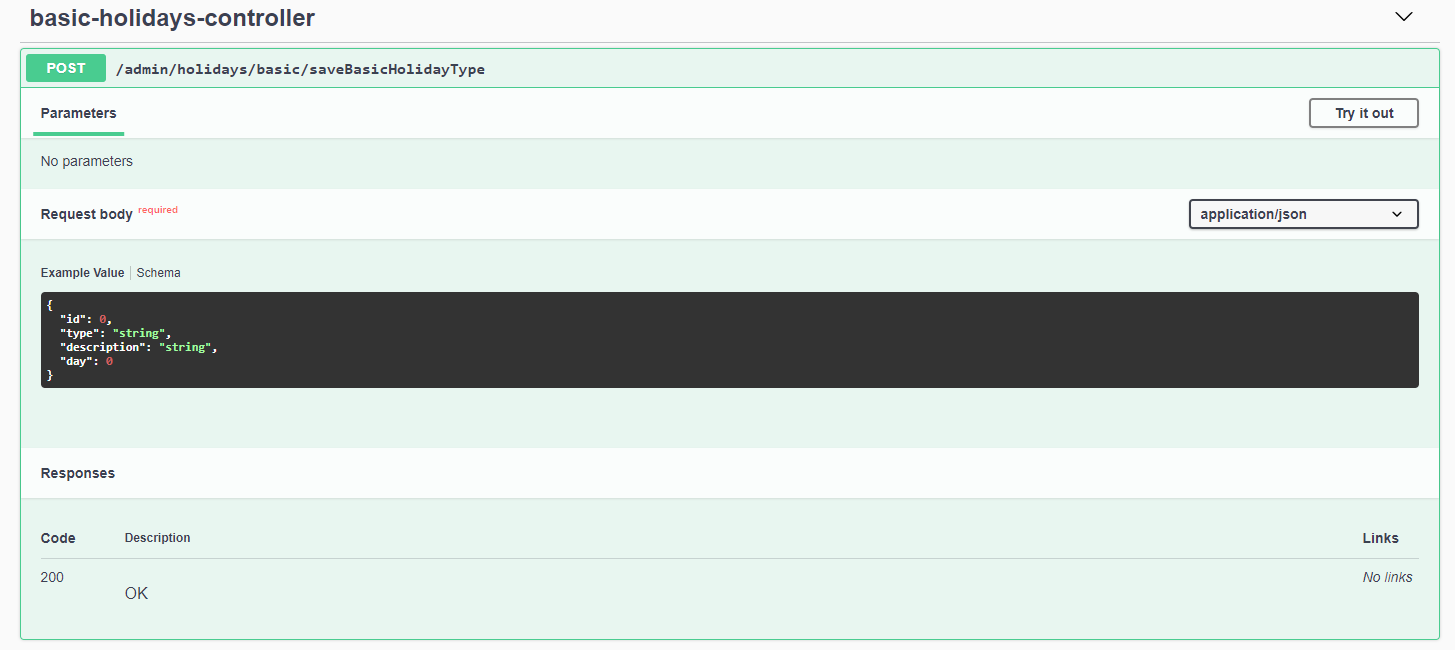
\includegraphics[scale=0.3]{images/swaggerPost.png}
	\caption{Swagger UI Post hívás tesztelése.}
	\label{fig:swaggerPostTest}
\end{figure}

\begin{figure}[h]
	\centering
	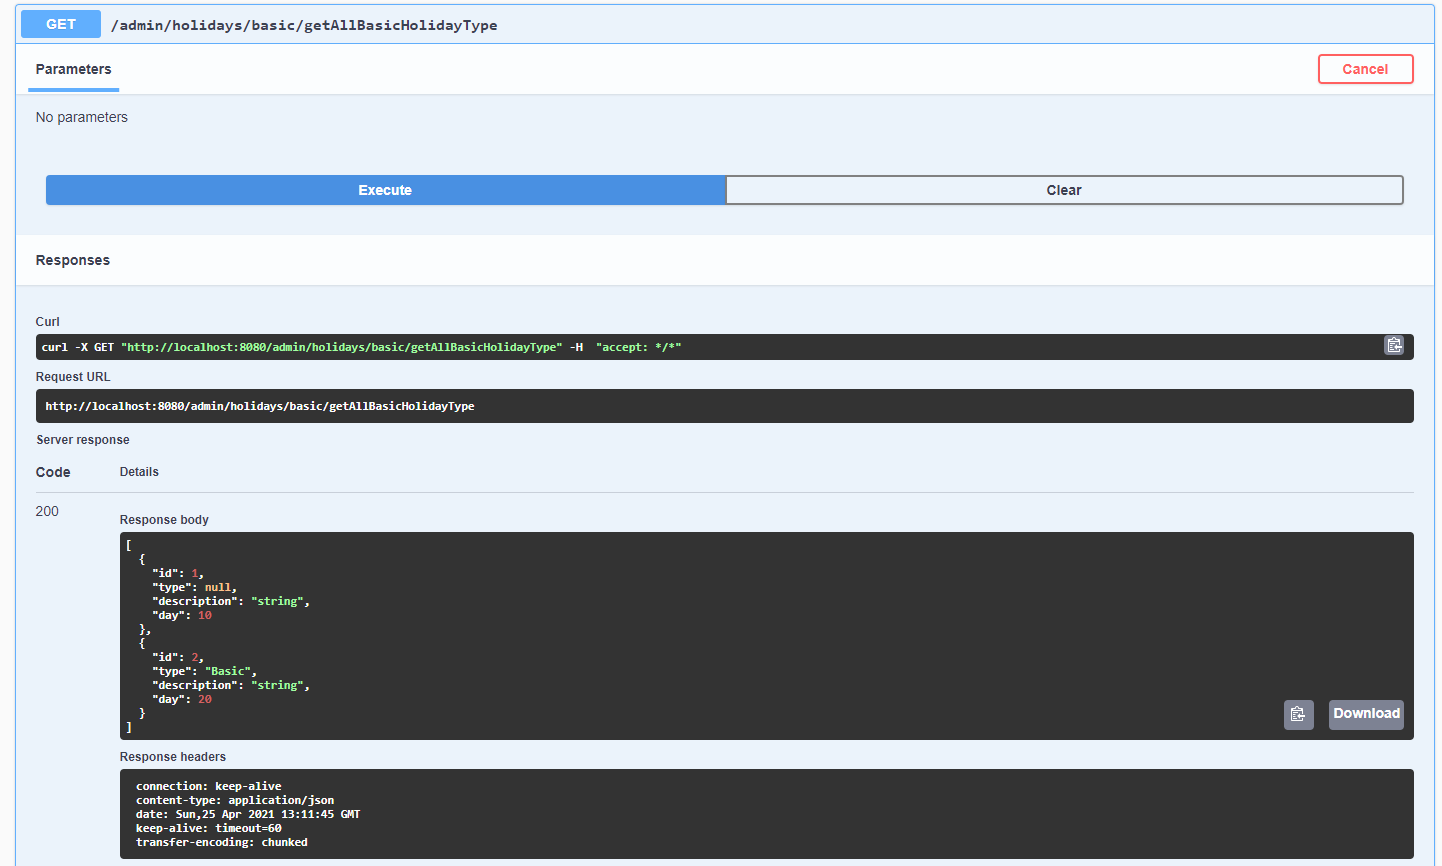
\includegraphics[scale=0.3]{images/swaggerGet.png}
	\caption{Swagger UI Get hívás tesztelése.}
	\label{fig:swaggerGetTest}
\end{figure}
\Chapter{Összefoglalás}

A szakdolgozatom elkészítését nagyban segítette, a Java Enterprise környezetben elsajátított szakmai tapasztalatom a webalkamázasokkal kapcsolatban. A kutatómunka, és a téma megismeréséhez szükséges előkészületek igen hasznos tudást nyújtottak a munkajog terén, valamint a komolyabb szoftvertervezéssel kapcsolatos ismereteimet is sikerült bővítenem. Az implementáció hosszas folyamata során kifejezetten sok új és hasznos szakmai ismeretanyagra tettem szert.

A program jelenlegi állapotában működőképes, de a teljes funkciókövetelménynek nem sikerült eleget tenni, így bőven tartalmaz még magában fejlesztési lehetőséget.

\Section{Fejlesztési lehetőségek}

Mivel több követelmény nem teljesült ezért több lehetőséget is szeretnék kifejteni, de mindezek előtt a továbbfejlesztésben az architektúra újragondolását tartom a legnagyobb lehetőségnek.
\paragraph{Architektúra} szempontjából, a microservice irányában folytatnám a program fejlesztését, melyet az adatbázis, és a megjelenítési réteg önállósításával lehet elkezdeni. így a központi logika összetettsége csökkenne, és a kódbázisok külön fejleszthetőek lennének.

\paragraph{A Statisztika generálás} funkcióra külön alkalmazást építenék, amely nem az összetett szabadságolással foglalkozó webalkalmazás egy modulja, hanem egy önállóan fejleszthető és karbantartható egység.

\paragraph{A szoftverbiztonság} szempontjából, a Spring által támogatott és egyetemeken is alkalmazott LDAP integráció fejlesztése. Ezzel a fejlesztéssel felhasználó szempontból megkönnyítjük a használatot, adatbázisunk csak és kizárólag a számunkra hasznos adatokat tárolná.

\paragraph{Kérelem jóváhagyás} esetén a már említett Flowable könyvtár használatával komolyabb utánajárást követően lefejleszthető.

A felsorolt fejlesztési lehetőségeken mellett a már specifikált, de még nem megvalósított részleteket mint például az éves terv generálása, valamint a megjelenítési réteg teljes implementálása természetesen előnyt élvez a fejlesztési sorban.



\clearpage

\addcontentsline{toc}{chapter}{Irodalomjegyzék}
\Urlmuskip=0mu plus 1mu\relax
\bibliographystyle{plain}
\bibliography{dolgozat.bib}

\newpage

\pagestyle{empty}

\noindent \textbf{\Large Adathordozó használati útmutató}

\vskip 1cm

Ez jellemzően csak egy fél-egy oldalas leírás.
Arra szolgál, hogy ha valaki kézhez kapja a szakdolgozathoz tartozó CD-t, akkor tudja, hogy mi hol van rajta.
Jellemzően elég csak felsorolni, hogy milyen jegyzékek vannak, és azokban mi található.
Az elkészített programok telepítéséhez, futtatásához tartozó instrukciók kerülhetnek ide.

A CD lemez tartalma
\begin{itemize}
\item a \texttt{dolgozat.pdf} fájl,
\item a \textbf{dolgozat\_latex} mappa tartalmazza a LaTeX forráskódját a dolgozatnak,
\item a \textbf{program} mappa tartalmazza az elkészített program forráskódját
\end{itemize}

\vskip 1cm

A program futtatásához a következő előfeltételek szükségesek:
\begin{itemize}
	\item A futtató számítógépre telepített Docker környezet
	\item Legalább Java 11-es verzió.
	\item Configurált Maven
	\item Node.js
	\item Angular.js
\end{itemize}

Az előfeltétel teljesítése után a következő parancsokkal indítható a program.

\begin{itemize}
	\item a holiday\_registry könyvtárban állva console-ban kiadjuk az \textbf{mvn clean install} parancsot
	\item a Frontend demo indításához a frontend mappában consoleon keresztül kiadjuk az \textbf{ng serve} parancsot (Ezután a localhost:4000 portján elérhető az oldal)
	\item a docker könyvtárban consoleból kiadjuk a \textbf{docker-compose up} parancsot.
	\item a Backend applikáció futásához a web könyvtárból kiandjuk az \textbf{mvn spring-boot:run} parancsot a program felülete a http://localhost:8080/swagger-ui/ linken elérhető.
\end{itemize}

\end{document}
